\documentclass[twoside,english]{uiofysmaster/uiofysmaster}

\usepackage[toc,titletoc,title,page]{appendix} %to add appendices (and have them in toc)
\usepackage[utf8]{inputenc}
%\usepackage{mhchem} %latex chemistry symbols
\usepackage{blindtext} %to fill in dummy text
%\usepackage{cite} %to have multiple citations in one \cite{key1,key2,..} -do not use with natbib!!
\usepackage{tcolorbox} %to have boxes w color around text and math mode
\usepackage{enumitem} %to reduce vertical spacing in enumerate
\usepackage{tabu} % to set tables to page width
%\usepackage{aas_macros}

\usepackage[sort&compress,square,comma,numbers]{natbib} %to use \citet, now mixed with [nr]
\usepackage[nottoc]{tocbibind}

\usepackage{float} 
\usepackage{pdfpages}
\usepackage{tikz}
\usetikzlibrary{arrows, shapes.callouts}
\tikzset{
    level/.style = { ultra thick, black },
    connect/.style = { dotted, black },
    notice/.style = { draw, rectangle callout, callout relative pointer={#1} },
    label/.style = { text width=2cm }
}
\usepackage{stackengine}

%---

\interfootnotelinepenalty=10000 % to force footnotes to NOT run over to the next page

%---
% to reduce space around table of contents (to fit everything into one page): 
\usepackage{tocloft}
\setlength{\cftbeforetoctitleskip}{0pt}
\setlength{\cftaftertoctitleskip}{0pt}
%---

\usepackage{epigraph}
\setlength\epigraphwidth{11cm}
\setlength\epigraphrule{0pt}

%---
\newcommand{\Sm}{$^{140}$Sm} % making it faster to write Sm140
\newcommand{\Pb}{$^{208}$Pb} 
\newcommand{\bd}{$\beta$-decay} % making it faster to write 
\newcommand{\ga}{$\gamma$}

%---
% modifying color in code listings and some style
%\usepackage{color}

% The predefined color names are: 
% black, blue, brown, cyan, darkgray, gray, green, lightgray, lime, magenta, olive, orange, pink, purple, red, teal, violet, white, yellow.
 
%\definecolor{codegreen}{rgb}{0,0.6,0} % too flashy
\definecolor{codegreen}{rgb}{0.0, 0.42, 0.24} % less flashy so comments not take all attention
\definecolor{codegray}{rgb}{0.5,0.5,0.5}
\definecolor{codepurple}{rgb}{0.58,0,0.82}
%\definecolor{codepurple}{rgb}{1.0, 0.0, 0.22} %carminered, could try it 
%\definecolor{backcolour}{rgb}{0.95,0.95,0.92} % original suggestion
\definecolor{backcolour}{rgb}{0.94, 0.97, 1.0}% aliceblue, not so flashy and not as ugly
\definecolor{LightGray}{gray}{0.95}
 
\lstdefinestyle{mystyle}{
    backgroundcolor=\color{backcolour},   
    commentstyle=\color{codegreen},
    %commentstyle=\color{codegray},    
    keywordstyle=\color{magenta},
    numberstyle=\tiny\color{codegray},
    stringstyle=\color{codepurple},
    basicstyle=\footnotesize,
    breakatwhitespace=false,         
    breaklines=true,                 
    captionpos=b,                    
    keepspaces=true,                 
    %numbers=left,     %removing line numbers in the code snippets               
    %numbersep=5pt,                  
    showspaces=false,                
    showstringspaces=false,
    showtabs=false,                  
    tabsize=2,
    %float=tp,
    %floatplacement=tbp
}
 
\lstset{
	style=mystyle,
	literate={~} {$\sim$}{1}
}
\renewcommand{\lstlistingname}{Code}
%---

%---
% new tcolorbox environment
% #1: tcolorbox options
% #2: color
% #3: box title
\newtcolorbox{mybox}[3][]
{
  colframe = #2!25,
  colback  = #2!10,
  coltitle = #2!20!black,  
  title    = #3,
  #1,
}

%---


%\bibliography{references}

\author{Trond Wiggo Johansen}
\title{Coulomb excitation of $\textnormal{\Sm}$}
\date{September 2019}
 
% ----------------------------------------------------------------------------------------------------------------------
% ----------------------------------------------------------------------------------------------------------------------
%Equations
%
%The command \eqref{} works exactly like \ref{}, but it adds parantheses to a plain number.
%
%Figures and tables
%
%\autoref{} is a usefull command when refering to to figures and tables. The command creates a reference with additional text corresponding to the target's type. For example, the command \autoref{fig:myfigure} would create a hyperlink to the \label{fig:myfigure} command, wherever it is. Assuming that this label is pointing to a figure, the hyperlink would contain the text "Figure 1.1", or similar.

%Two basic citation commands, \citet and \citep for textual and parenthetical citations, respectively. …
%\citet{jon90} --> Jones et al. (1990)
%\citep{jon90} --> (Jones et al., 1990)
%\citet*{jon90} --> Jones, Baker, and Williams (1990)
%\citep*{jon90} --> (Jones, Baker, and Williams, 1990)


\begin{document}

% set space around equations
\setlength{\belowdisplayskip}{12pt} \setlength{\belowdisplayshortskip}{12pt}
\setlength{\abovedisplayskip}{12pt} \setlength{\abovedisplayshortskip}{12pt}

\maketitle

%Centering the front page, see: https://github.com/ComputationalPhysics/uiofysmaster

%%% ABSTRACT
\begin{abstract}


\end{abstract}


\begin{dedication}
To my family, for all their support and encouragement!

\end{dedication}

\begin{acknowledgements}
Supervisors Andreas Görgen and Katarzyna Hady\'nska-Kl\c ek

Nuclear Physics Group

Computational Physics Group, Morten Hjorth-Jensen

CERN-ISOLDE, Liam Gaffney

Lillefy, FFU, Fysikkforeningen

My family

Morten, Alex and Astrid.

Ina, for pushing me towards excellence, I love you.

\subsection*{Collaboration details}



ENSAR2: European Nuclear Science and Applications Research - 2 \url{http://www.ensarfp7.eu}, UiO, ISOLDE, other contributors to the experiment?

  \vspace{1.5cm}
  
  \noindent\textit{Trond Wiggo Johansen}\\
  
  \noindent September, 2019
  
\end{acknowledgements}


\tableofcontents


% ----------------------------------------------------------------------------------------------------------------------
% ----------------------------------------------------------------------------------------------------------------------

\chapter{Introduction}
\textcolor{red}{+ Motivation}


kinsim \cite{kinsim}

The experiment has been done before, with lower energy (and another target), Malin Klintefjord. \url{http://urn.nb.no/URN:NBN:no-56121} \newline
 
 
Experiment conducted 8th - 14th of August 2017.

\bigskip

\textcolor{Magenta}{Tilbakemelding: \newline 
old REX-ISOLDE post-accelerator limited to 2.8 MeV/u (low Coulomb excitation cross section, low probability for multi-step excitation). Mo target was chosen to maximize cross section at this energy, and to normalize B(E2; $0^+ \rightarrow 2^+$) value in \Sm ~to the well-known B(E2) value for the target. \newline
New HIE-ISOLDE: energies up to 10 MeV/u $\implies$ we can choose high-Z target (Pb) $\implies$ high Coulex cross section, especially for multi-step. Also: B(E2) for \Sm ~now known from previous experiment (and a lifetime measurement) $\implies$ no need for normalization: we can use the known B(E2; $0^+ \rightarrow 2^+$) to nomalize the transition probabilities for the higher-lying transitions. Chosen 4.7 MeV/u as the highest possible energy that is safe for Pb (distance of closest approach large enough to exclude nuclear interaction.)}


% ----------------------------------------------------------------------------------------------------------------------
% ----------------------------------------------------------------------------------------------------------------------

\chapter{Theory}

Quadrupole deformation of nuclei. \newline

Shape coexistence possible for certain regions of $N$ and $Z$.

\bigskip

- triaxial shape / shape coexistence \newline
- benchmark for theoretical models \newline
- transition probabilities and quadrupole moments between several excited states are not known \newline
- fundamental research

\bigskip

COULEX: \newline
- nucleus excited by electromagnetic interaction. \newline
- de-excitation $\rightarrow$ gamma

\bigskip

\textcolor{Magenta}{Tilbakemelding: \newline 
shape coexistence often found near closed shells. Example: neutron deficient Hg nuclei (Z = 80 just below 82 shell closure, N $\sim$ 104: neutron mid-shell). \newline
\Sm: N = 78, just below N = 82 shell closure, Z = 62: mid-shell. \newline
Typical indication for shape coexistence: $0^+$ states (often at low energy). \newline 
\Sm ~was thought to have a low-lying $0^+$ state [Firestone], but this state was shown to be $2^+$ [Suoranczyk?]. Indication for $0^+$ states around 1.5 MeV. \newline 
One of the objectives of this experiment: clarify the nature/structure of these $0^+$ states. \newline 
Shape transition: Sm-144 (Z = 62, N = 82) spherical. Adding neutrons: transition of N = 90 from spherical to prolate deformed $\rightarrow$ shape-phase transition, so called X(5) critical-point symmetry. \newline
Taking out neutrons: very neutron-deficient Sm nuclei are also prolate deformed (e.g. Sm-132), but for \Sm: indication for triaxiality/\ga-softness [Klintefjord] $\rightarrow$ another form of shape-phase transition/critical point behavior $\implies$ E(5) [Iachello?]. \Sm ~could be one of the best examples for E(5) symmetry $\implies$ need transition probabilities from higher-lying states to confirm.} \newline


\textcolor{red}{Some suggestions:} \newline
$\bullet$ general things about nuclei shapes \newline
- multipole expansion, shape parameters (5 parameters, 3 for space, 2 for deformation $\beta$, \ga), ... \newline
- quadrupole moments: intrinsic (body-fixed frame), spectroscopic (lab frame)  \newline
- transition probabilities, el.magn. matrix elements  \newline
- rotations and vibrations $\rightarrow$ energy spectra, B(E2) values  \newline
- Casten triangle (spherical vibrator, deformed rotor, \ga-soft + X(5), E(5)), expected spectrum for E(5) nuclei \newline

$\bullet$ the basics of Coulomb excitation 

% ----------------------------------------------------------------------------------------------------------------------
% ----------------------------------------------------------------------------------------------------------------------
\newpage

\chapter*{\textcolor{red}{NOTES TO BE REMOVED!!}}
\section{Oppgaveteksten (skal fjernes!)}
\textcolor{red}{---------} \newline
\textcolor{red}{Oppgavens mål:} \newline
The ISOLDE facility at CERN has been upgraded to provide higher energies and intensities for radioactive ion beams. A new experiment to study 140Sm was performed in the summer of 2017. The goal of the experiment was to measure electromagnetic transition probabilities and electric quadrupole moments for several excited states in 140Sm by measuring Coulomb excitation probabilities. A large data set was obtained using silicon detectors to determine the energies and angles of scattered particles, and germanium detectors to measure gamma rays from excited states in 140Sm. \newline

The goal of the master thesis is to analyze the data from this experiment. The required tasks include development and improvement of data analysis software to determine Coulomb excitation yields. These yields will then, in a second step, be compared to theoretical calculations and transition probabilities and quadrupole moments will be extracted using chi-square minimization procedures. \newline


\textcolor{red}{Prosjektbeskrivelse (omfang 60 studiepoeng):} \newline
The shape of an atomic nucleus is determined by a delicate interplay between macroscopic (liquid drop) properties and microscopic shell effects. Nuclei with filled proton or neutron shells (i.e. magic nuclei) are generally spherical in shape, whereas nuclei with open shells gain energy by assuming a deformed shape. Depending on the occupation of specific orbitals, the nuclear shape can change drastically by adding or removing protons or neutrons. Certain nuclei exhibit shape coexistence, i.e. the coexistence of quantum states that correspond to different shapes. Because the shape of a nucleus is so sensitive to the underlying nuclear structure and to changes of the proton and neutron numbers, the excitation energy, or the angular momentum, observables related to the nuclear shape are used as benchmarks for theoretical models. 

Nuclei in the rare earth region, and in particular the chain of samarium isotopes, exhibit a variety of shape effects. The Sm isotope with closed neutron shell at N=82, 144Sm, is spherical in shape. Adding neutrons to 144Sm changes the deformation to an elongated (prolate) quadrupole shape. The transition from spherical to prolate shape, which occurs for 152Sm at N=90, can be interpreted as a shape-phase transition. Flattened (oblate) quadrupole shapes are predicted by theory to occur below the N=82 shell closure. An earlier experiment studying 140Sm at CERN-ISOLDE found triaxial shape for this isotope, i.e. a shape where all three principal axes of the ellipsoid have different lengths. 140Sm can therefore be considered to lie at the critical point of a phase transition from spherical to deformed, and from prolate to oblate shape. \newline

\textcolor{red}{Foreløpig tittel:} \newline
Coulomb excitation of 140Sm \newline


\textcolor{red}{Metoder som tenkes benyttet:} \newline
Multi-step Coulomb excitation with radioactive beam, isotope separation on-line technique, nuclear spectroscopy, particle-gamma and particle gamma-gamma coincidence analysis, advanced chi-square minimization procedures. \newline
\textcolor{red}{---------} \newline


\section{Information sources}
\begin{itemize}  
\item CD: \url{https://www.ikp.uni-koeln.de/~warr/doc/cd.pdf}
\item Why CoulEx? \url{https://iks32.fys.kuleuven.be/wiki/brix/images/5/58/10_20151123_Illana_BriX15_web.pdf}
\item 2017: \url{https://iopscience.iop.org/article/10.1088/1361-6471/aa5c4e#jpgaa5c4es2}
\item 2017: \url{http://iopscience.iop.org/article/10.1088/1361-6471/aa990f/pdf}
\item \url{http://publications.lib.chalmers.se/records/fulltext/175494/local_175494.pdf}
\item \url{https://www.euroschoolonexoticbeams.be/site/files/nlp/LNP700_contrib2.pdf}
\item 2004: \url{http://accelconf.web.cern.ch/AccelConf/e04/PAPERS/TUXCH01.PDF}
\item 2003: \url{https://ac.els-cdn.com/S0168583X02018864/1-s2.0-S0168583X02018864-main.pdf?_tid=64f42a8d-b37c-42a6-a3c5-f01dcee73366&acdnat=1545049646_8918b985af428e17c9741f7142fe0e36} 
\item 2002: \url{https://ac.els-cdn.com/S0168900201009548/1-s2.0-S0168900201009548-main.pdf?_tid=71a410a3-6554-4268-ac1a-1b43cae4039d&acdnat=1545056166_15ff5318affd89c7e63f819c9229a9e9}
\end{itemize}

\bigskip

Post-accelerated beams ISOLDE \url{http://iopscience.iop.org/article/10.1088/1361-6471/aa78ca}

\bigskip

PSB \url{https://home.cern/science/accelerators/proton-synchrotron-booster}


\section*{\textcolor{red}{Sjekk sensorveiledning!!}}


\newpage

% ----------------------------------------------------------------------------------------------------------------------
% ----------------------------------------------------------------------------------------------------------------------

\chapter{Coulomb excitation experiment} 


\section{ISOLDE at CERN}
The acronym ISOLDE stands for Isotope Separator On Line DEvice. ISOLDE is a Radioactive Ion Beam (RIB) facility at CERN in Meyrin, Switzerland.  \autoref{fig:accelerators} shows the CERN accelerator complex \cite{CERN-AC}, where ISOLDE is located beside the Proton Synchrotron Booster (PSB). The facility can produce over 1000 different radionuclides to be used in a wide variety of experiments in nuclear physics, atomic physics, solid state physics, life sciences and fundamental interactions. Experiments have been performed at ISOLDE since 1967 and since 2001 experiments with post-accelerated RIBs have been conducted. The high intensity and energy upgrade (HIE-ISOLDE) have made it possible to deliver energies up to 10 MeV/$u$ in 2018 \cite{HIE-ISOLDE, ISOLDE-web, ISOLDE-facility}. 

Most of the around 4000 known nuclides are radioactive. In many cases it is not possible to make radioactive nuclei targets and perform an experiment because of the short half-life of the nucleus of interest. To study these radioactive nuclei, RIBs are used on stable targets. One way of obtaining a RIB is to use the Isotope Separator On Line (ISOL) method. In the ISOL method, two accelerator systems is needed. The first accelerator is used to produce the radioactive atoms at rest, and the second accelerator is used to accelerate these atoms \cite{ISOL}. 

\begin{figure}[t]
	\centering
	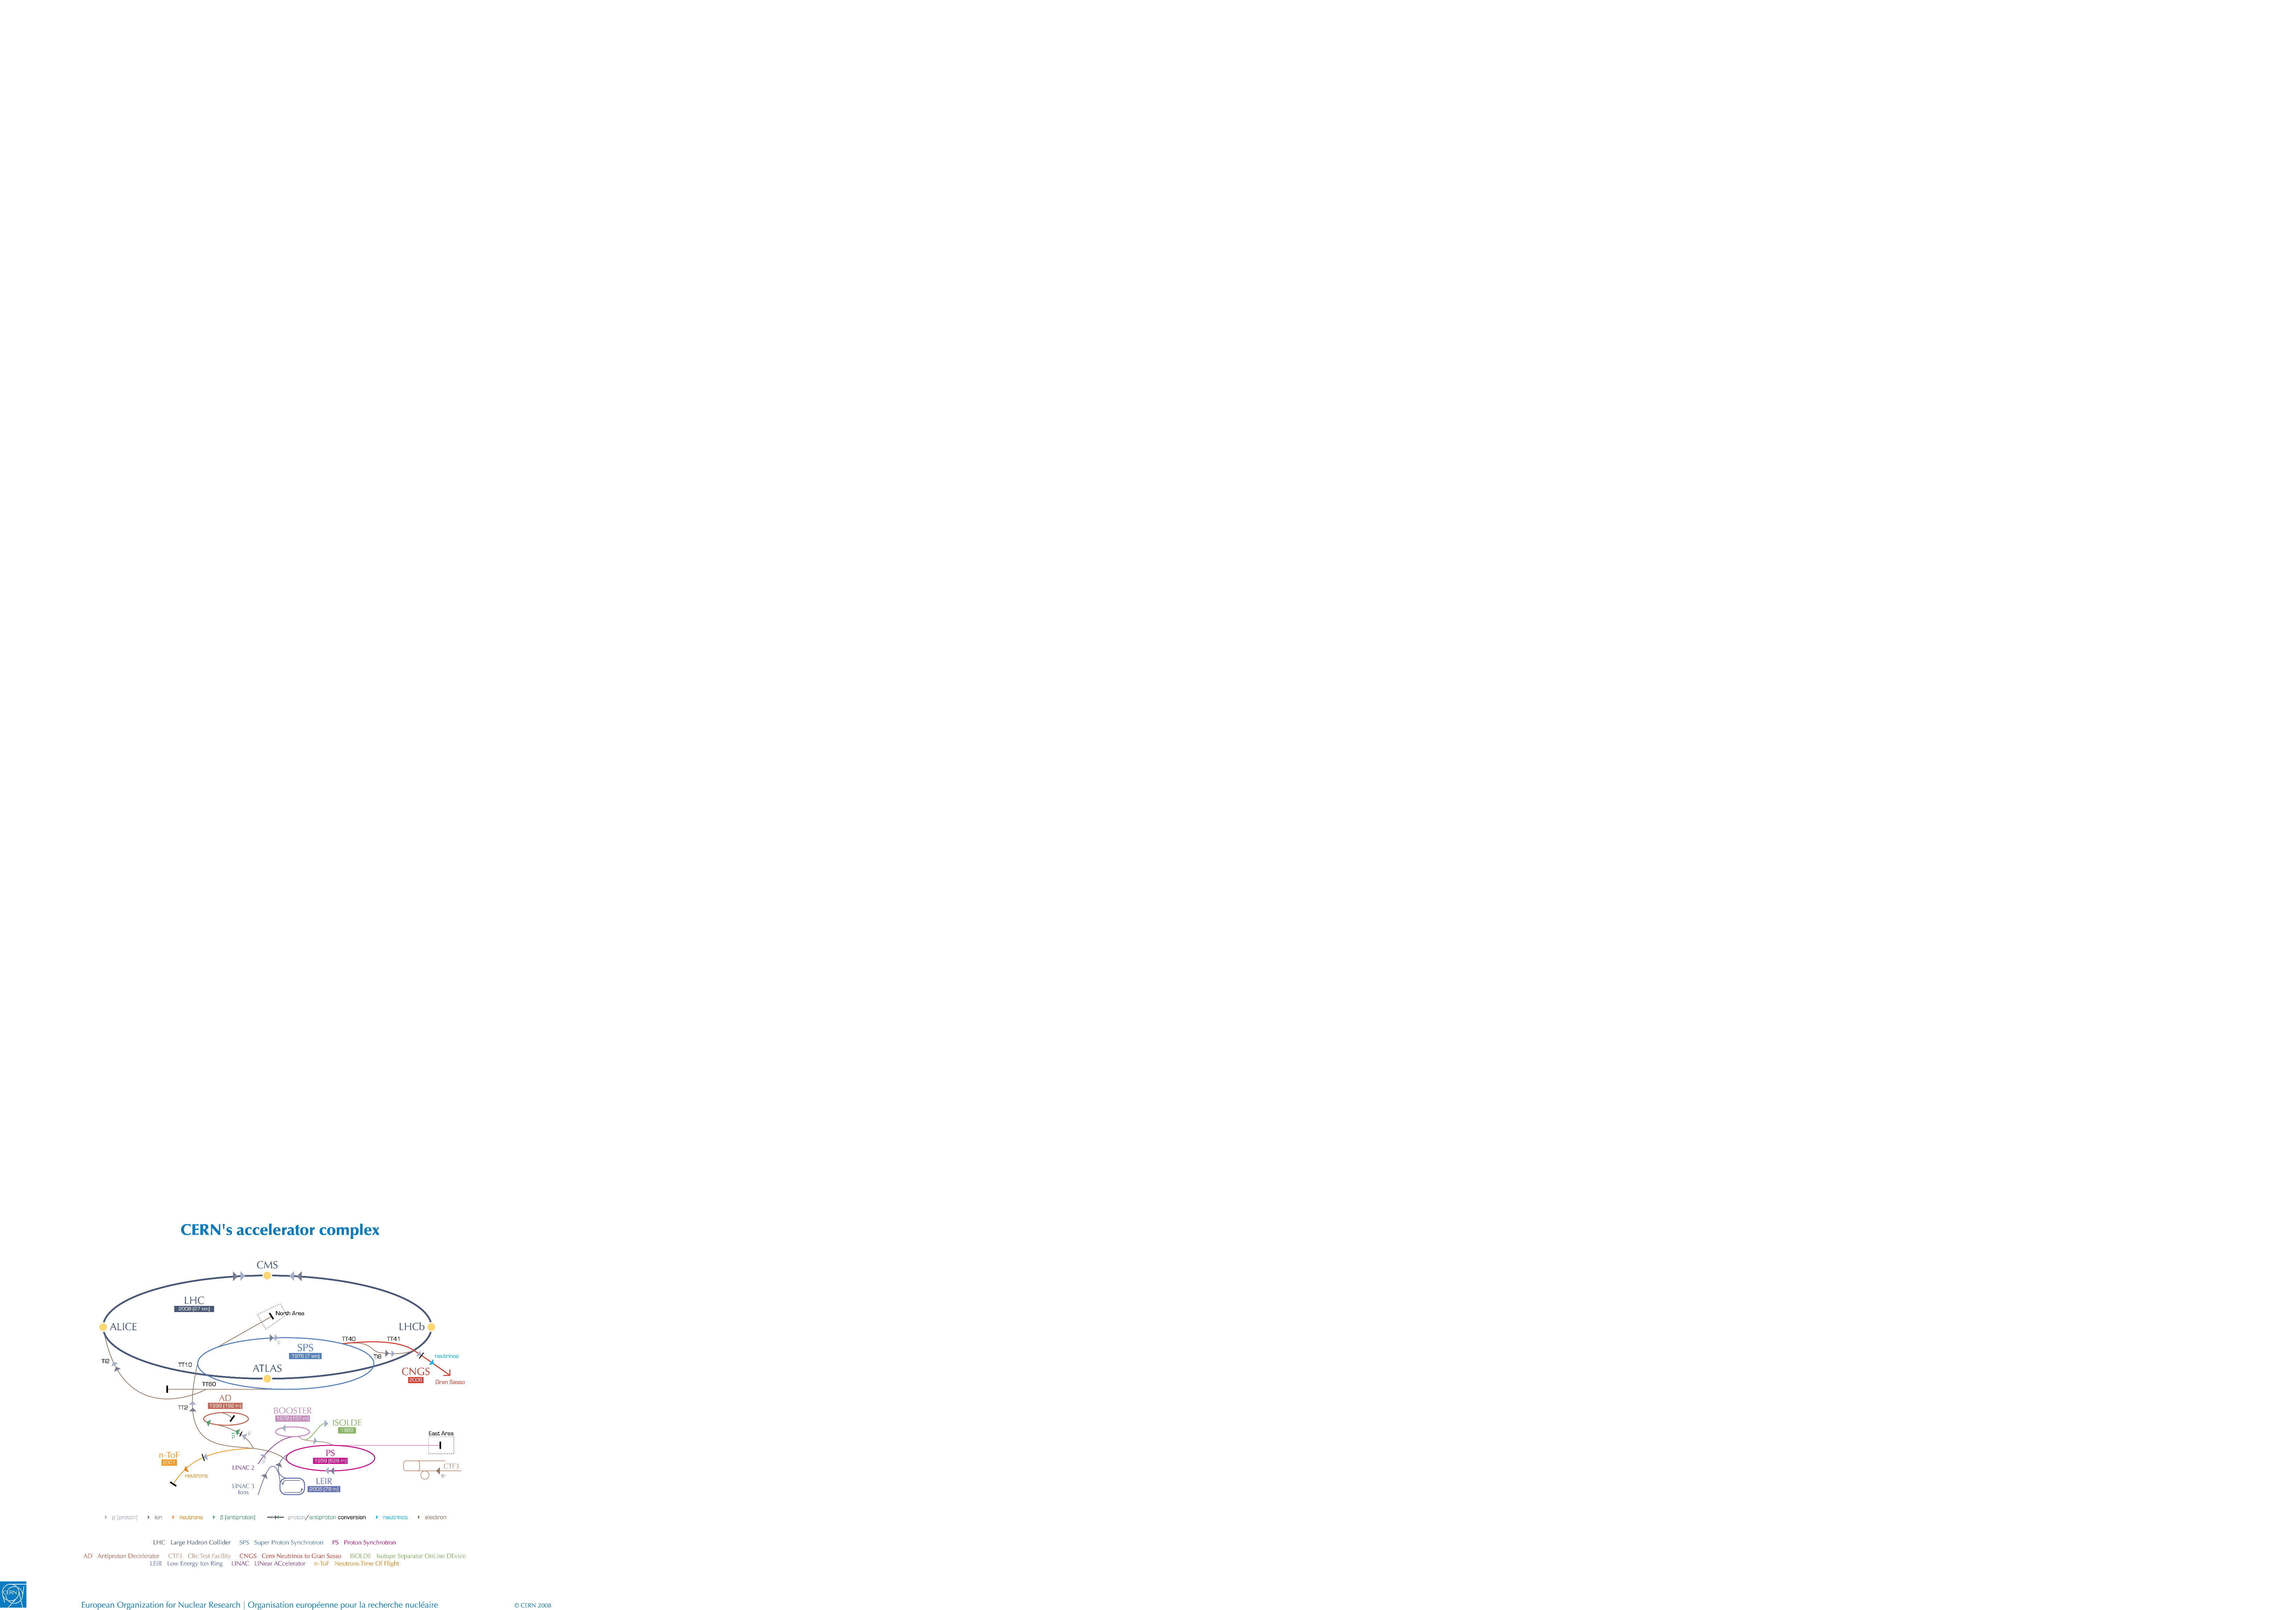
\includegraphics[width=\textwidth]{images/0812015.pdf}
	\caption{The CERN accelerator complex. ISOLDE gets accelerated protons from LINAC 2 and the PS BOOSTER.}
	\label{fig:accelerators}
\end{figure}


\subsection{Beam production}
A continuous flow of accelerated proton beam bunches from the PSB comes into the ISOLDE facility and collide with a thick production target. The proton beam has an energy of 1.4 GeV and an intensity up to 2 $\mu$A. Two proton beam bunches is separated by 1.2 s. ISOLDE typically takes 50\% \textcolor{red}{\textbf{REF?}} of all proton bunches form the PSB, the rest goes to the LHC and other experiments shown in \autoref{fig:accelerators}. In the reaction between the proton beam and the production target, radioactive nuclides are produced in spallation, fission or fragmentation reactions (basically smashing the target into pieces) \cite{ISOLDE-web}. The production target is chosen from a stable region heavier than the nucleus of interest. In our experiment, a production target of tantalum (Ta) was used, producing the elements in the chart of nuclides up to tantalum. A large amount of different isotopes is produced in this way, and the challenge is to extract the nucleus of interest. 
 
\textcolor{red}{find other refs as well! forklare figuren mer?}


\bigskip

\textcolor{Magenta}{Tilbakemelding: \newline 
A large amount of different nuclei/isotopes is produced in this way. Challenge: extract the nuclei we are interested in. Idea: selective ionization $\rightarrow$ use HV (electrostatic field) to extract Sm ions electronic transitions are characteristic for each chemical element. use laserlight to excite an electron to a specific excited (electron) state in Sm, use another laser to excite electrons further to another excited state, 3. laser to to kick out the electron $\rightarrow$ only Sm atoms are ionized. There could be contaminants from surface ionization (atoms that collide with the walls of the ion source).}

*bruker laser on/off for å se hva annet som kommer ut av beamen


\textcolor{red}{RILIS:} \newline
The resonance ionization laser ion source (RILIS) is based on the method of step-wise excitation and ionization of the atom. It is an element-selective process which is used to produce ion beams of the correct element \cite{RILIS}. In this experiment RILIS was used to select samarium with atomic number $Z = 62$. 

* 2-3 step ionization
* also other elements come through

\textcolor{red}{Other refs:} \url{http://rilis.web.cern.ch} and \url{https://www.research.manchester.ac.uk/portal/files/60831252/FULL_TEXT.PDF} and \url{https://www.sciencedirect.com/science/article/pii/S0168583X13008914?via%3Dihub}

\bigskip

\textcolor{red}{GPS:} \newline

\textcolor{Magenta}{Tilbakemelding: \newline 
at this point we have a continuous beam of Sm ions of 60 keV energy (the target is on a 60 kV HV platform). \newline
next step: we need to have mass separation, and we need to give this continuous beam a fine structure, because the post-accelerator cannot accept a continuous beam coming in, it also accelerates bunches.}

The beam can collide in one of two target stations, either the general purpose separator (GPS) or the high resolution separator (HRS). The GPS has one bending magnet and can deliver beams of different masses simultaneously into three beam lines, while the HRS has two bending magnets with high mass resolving power which delivers the beam into the main beam line \cite{GPS}. In this experiment the GPS was used to select the isotope of samarium with mass number $A = 140$. 

\textcolor{Magenta}{Tilbakemelding: \newline
now we have a continuous beam of \Sm. The mass separator gets also rid of contaminants that come out of RILIS but have different mass. There could still be isobaric contaminants from surface ionization but luckily there is very little surface ionization for the neighboring elements of Sm. Laser ON/OFF.}

\textcolor{red}{Other refs:}  \url{http://isolde.web.cern.ch/targets-and-separators} and \textcolor{purple}{Klintefjord's PhD}

\bigskip

\textcolor{red}{REXTRAP:} \newline
REXTRAP is a penning trap which has the tasks of accumulation, bunching and cooling of the RIB. \cite{HIE-ISOLDE} The ions are released in bunches and transfered to the REXEBIS.

\textcolor{Magenta}{Tilbakemelding: \newline 
In REXTRAP we collect the \Sm ~ions, so that we can release them in bunches that are matched to the fine structure of the LINAC.}


\textcolor{red}{Other refs:} \url{https://www.sciencedirect.com/science/article/pii/S0168900204020169} and \url{https://www.sciencedirect.com/science/article/abs/pii/S0375947401016426}

\bigskip

\textcolor{red}{REXEBIS:} \newline
REXEBIS is a charge breeder where the RIB is bred to a high charge state \cite{REXEBIS}, with a mass-to-charge ($A/q$) ratio typically between 2.5 and 4.5 \cite{Post-acc}. REXEBIS releases the beam with a certain energy through a mass separator and into the HIE-ISOLDE LINAC (LINear ACcelerator) \cite{HIE-ISOLDE}. 

\textcolor{Magenta}{Tilbakemelding: \newline
go from \Sm$^{+1}$ to \Sm$^{+33}$ (I think, check log book), anyway we need a highly charged ion to accelerate to high energies. The electron beam of EBIS just blasts off more electrons from Sm. The longer the ions stay in EBIS, the higher the charge state $\rightarrow$ distribution of charge states $\rightarrow$ we loose those that have the wrong charge state. LINAC can only accept one.}

\textcolor{purple}{excites the nucleus in three steps ionizing the atom, which leaves the nucleus in a high charge state.  ?}

\bigskip

\textcolor{red}{Other refs:} \url{http://cds.cern.ch/record/478399/files/} and \url{http://rex-isolde.web.cern.ch}


\textcolor{red}{HIE-ISOLDE LINAC:} \newline
The HIE-ISOLDE LINAC accelerates the beam through the beam line and magnets bend the beam into MINIBALL. 

* one of the first Miniball experiments with the new accelerator

\textcolor{Magenta}{Tilbakemelding: \newline
Accelerates \Sm ~to 4.65 MeV/u}

\bigskip

HIE-ISOLDE (Superconducting LINAC Upgrade): Linear accelerator, HIE-LINAC \newline

\bigskip

HIE-ISOLDE \url{http://hie-isolde-project.web.cern.ch}, technical design \url{http://cds.cern.ch/record/2635892?ln=en}, direct to doc: \url{http://cds.cern.ch/record/2635892/files/HIE-ISOLDE_TDR.pdf}


\textcolor{red}{MINIBALL:} \newline



\textcolor{red}{Cite: \url{https://ac.els-cdn.com/0168583X92959079/1-s2.0-0168583X92959079-main.pdf?_tid=0ccb0647-5870-48f9-ac38-df8c0077981c&acdnat=1545216224_d359ddcc40ea1f94369c85a141edba63} and \url{https://cds.cern.ch/record/2025701/files/epjconf_inpc2013_11005.pdf} and \url{http://isolde.web.cern.ch/targets-and-separators}}


\bigskip

Magnets....

\bigskip

ISOLDE actually uses the most protons at CERN [\textcolor{red}{ref?}].


ISOLDE \url{http://iopscience.iop.org/article/10.1088/1361-6471/aa5f03/pdf}

\bigskip

Very pure beam (\textcolor{red}{did we have statistics of this?}) - resultat til avhandling. sjekk etter doppler-korrigering. Nd-contaminasjon? i så fall veldig lite, 1-2 prosent?

\textcolor{Magenta}{Tilbakemelding: \newline
we would have to look at the \ga-spectra to identify any contaminants. There may be a little bit of Nd-140 in the beam, but if so, it is very little (judging from on-line spectra).}

\bigskip

MINIBALL \url{http://isolde.web.cern.ch/experiments/miniball} and \url{https://www.miniball.york.ac.uk/wiki/Main_Page}

\bigskip

ENSAR2 \url{http://www.ensarfp7.eu}

\bigskip

Beam production \url{http://tuprints.ulb.tu-darmstadt.de/4599/1/TUDthesis_Christoph%20Seiffert.pdf}

\bigskip

Test \cite{CERN-AC}, copyright: \url{https://copyright.web.cern.ch}

\bigskip

CERN Document Server  \url{https://cds.cern.ch}


\subsection{Target}

\textcolor{red}{Kan skrive om dette i motivasjonen.}

\Pb\ was chosen as a target. Want high $Z$ so that the probability of excitation is high. \newline

\textcolor{Magenta}{Tilbakemelding: \newline
Thickness, etc. \newline
It is very hard to excite \Pb ~(doubly magic). We might see a little bit of the 2.6 MeV state (octupole vibration), but not sure. \newline
Since we don't need normalization (because we have the B(E2, $0^+ \rightarrow 2^+$) from the previous experiment and from lifetime measurement [Bello], we have chosen a target that is very hard to excite, so transitions from the target will not complicate the spectrum.}

Doubly magic, very hard to excite. No quadrupole deformation/excitation. Need quadrupole for first state (see nndc)

ja og nei: Not enough beam energy to excite \Pb. \newline

Highest $Z$ for maximum excitation probability.


Contamination... finger print [\textcolor{red}{picture}]


\section{Miniball}

Testcite (Nigel Warr) \cite{NWarr}


Pictures \url{https://cds.cern.ch/record/844871?ln=en}

\subsection{Particle detector, DSSSD (CD)}

DSSSD: Double sided silicon strip detector

16 rings, 12 strips effectively (24 strips, 12 pairs with two strips making a pair)

Rings = annular strips, strips = radial strips or sector strips

CD distance: 26.98 mm, Inner angle (min): 9 mm, Outer angle (max): 40.9 mm

Angle coverage: [18.4$^\circ$, 56.6$^\circ$]

See \autoref{fig:ADC-FB}

\begin{figure}[ht]
	\centering
	\includegraphics[width=\textwidth]{images/cd_drawing.pdf}
	\caption{CD drawing, adapted from Nigel Warr.}
	\label{fig:ADC-FB}
\end{figure}


%\begin{figure}
%	\centering
%	\input{images/CD-geometry.tikz}
%	\caption{CD-geometry.}
%	\label{fig:CD-geometry}
%\end{figure}


See \autoref{tab:CD_angles}

\begin{table}[ht] \centering 
	% Data for the CD angles table
\begin{tabular}{ccccc}
\hline
Ring   & \multicolumn{2}{c}{Center of CD ring}                            &             &             \\
number & \shortstack{Distance from \\ beam line [mm]}  & Angle [$^\circ$] & $E_t$ [MeV] & $E_b$ [MeV] \\
\hline
1      & 10                                            & 20.3             & 484.86      & 539.89      \\
2      & 12                                            & 24.0             & 457.53      & 520.55      \\
3      & 14                                            & 27.4             & 428.87      & 499.72      \\
4      & 16                                            & 30.7             & 398.95      & 478.33      \\
5      & 18                                            & 33.7             & 369.54      & 456.71      \\
6      & 20                                            & 36.5             & 340.64      & 435.42      \\
7      & 22                                            & 39.2             & 313.65      & 414.84      \\
8      & 24                                            & 41.6             & 287.31      & 395.31      \\
9      & 26                                            & 43.9             & 262.77      & 376.35      \\
10     & 28                                            & 46.0             & 240.36      & 358.75      \\
11     & 30                                            & 48.0             & 219.53      & 342.40      \\
12     & 32                                            & 49.8             & 198.95      & 326.87      \\
13     & 34                                            & 51.5             & 182.41      & 312.31      \\
14     & 36                                            & 53.1             & 164.55      & 299.11      \\
15     & 38                                            & 54.6             & 151.51      & 286.78      \\
16     & 40                                            & 56.0             & 139.62      & 273.80      \\
\hline
\end{tabular}
\end{table}

\textcolor{red}{\textbf{SKAL TABELLEN VISE MeV eller MeV/u??}}

\textcolor{red}{Vis en figur/tegning av "trekanten" i detektoroppsettet? Skjematisk figur?} 

\begin{align*}
	\theta = \tan^{-1} \left( \frac{\text{opposite}}{\text{adjacent}} \right)
\end{align*}

\subsection{\texorpdfstring{$\gamma$}{Gamma} detectors, HPGe}

24 six-fold segmented. 8 clusters of 3 crystals each. Each crystal segmented in 6 parts (144 segments in total).

\bigskip

Cryo-modules

\section{Experimental setup}
\Sm ~Coulomb excitation experiment.

\begin{figure}[ht]
	\centering
	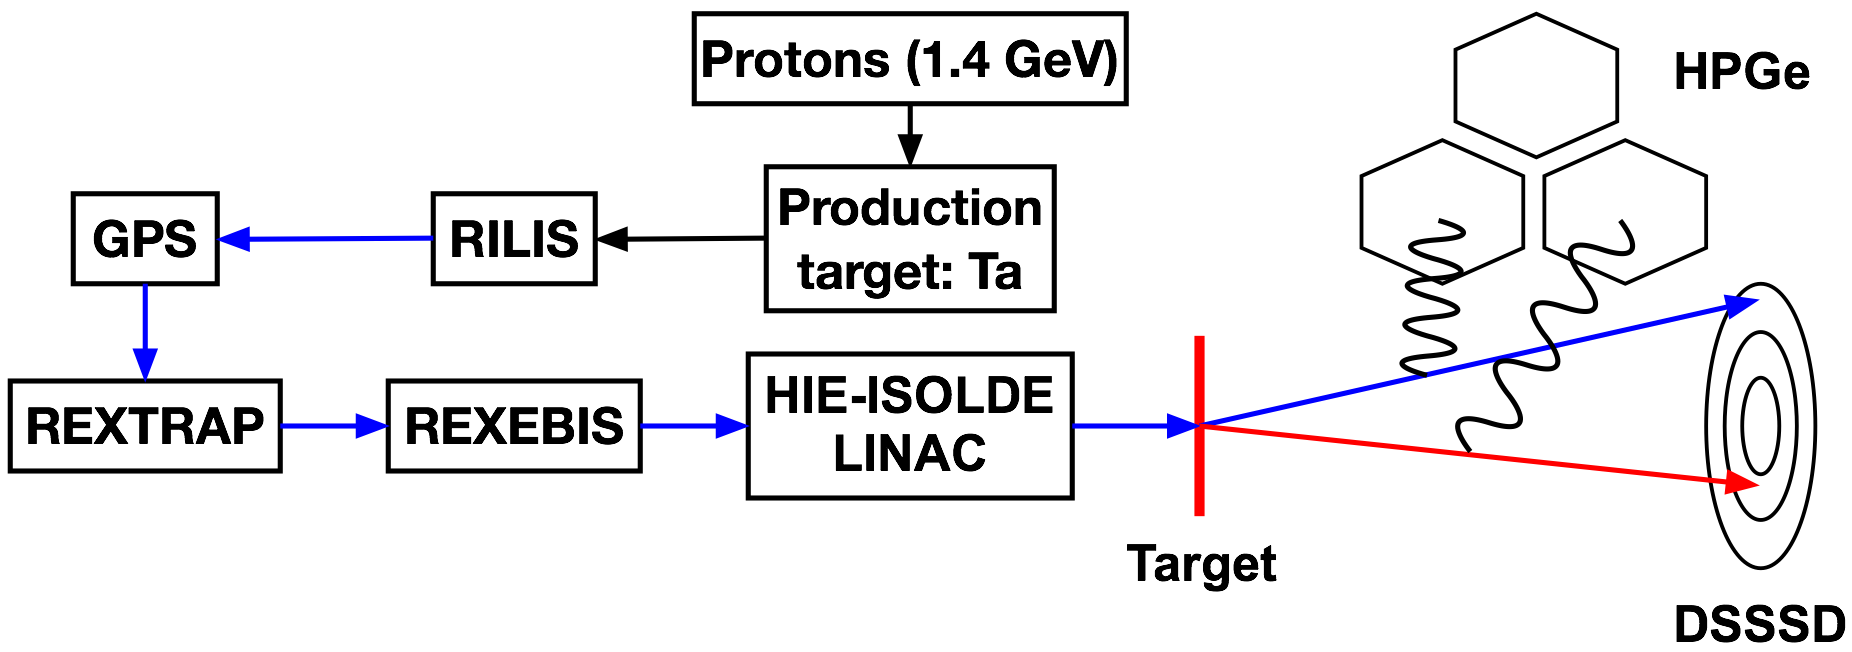
\includegraphics[width=\textwidth]{images/Coulex-ISOLDE.png}
	\caption{The Coulomb excitation setup at ISOLDE. Adapted from Malin Klintefjord's PhD thesis \cite{Klintefjord}.}
	\label{fig:Coulex}
\end{figure}

\textcolor{red}{Show where Sm is made + ionized (+1) + bred (+33 or +34?) in the figure?}

\bigskip

Experiment code: IS558 

Ta: tantalum (Z = 73)

Sm: samarium (Z = 62)

Pb: lead (Z = 82) \newline



Beam: \Sm ~(T$_{1/2} = 14.82$ min, 4.65 MeV/$u$, total 651 MeV), excellent purity

Target: \Pb ~(Thickness: 1.4 mg/cm$^2$)


Small angle: Forward scattering: Larger distance, weaker \textcolor{red}{EM}-field, less excitation probability.

Large angle: Backward scattering: Closer distance, stronger \textcolor{red}{EM}-field, higher excitation probability. \newline


\bigskip

Expect to measure transition probabilities $B(E2)$ and quadrupole moment (nuclear deformation). 

\bigskip



% ----------------------------------------------------------------------------------------------------------------------% ----------------------------------------------------------------------------------------------------------------------



\chapter{Data analysis}  

\textcolor{Magenta}{Tilbakemelding: \newline
First: explain the tasks and give the bigger picture of what needs to be done: \newline 
starting point: Raw data in list mode: ID, E, T, ID, E, T, ... (basically) \newline
what you want: Doppler-corrected $\gamma$-spectra with various conditions on particles, angles, etc. \newline
procedure: 3 steps: \newline 
1. convert raw data to ROOT format \newline
2. event-building: \newline
$\bullet$ calibrate detectors, apply thresholds, etc. \newline
$\bullet$ use correlations to build events: particle-$\gamma$ coincidences \newline
$\bullet$ store everything in a tree structure for easy access \newline
3. apply gates on particles and perform Doppler correction \newline
--------- \newline
Could be nice to have a ''cook book'', i.e. step-by-step explanation of this procedure.
}

\bigskip

ROOT: analysere data

kinsim3 \url{https://github.com/lpgaff/kinsim} + SRIM \url{http://www.srim.org}

\bigskip


\begin{table}[H] 
\centering 
\caption{Computer used for data analysis}
\label{tab:PC}
\begin{tabular}{ll}
\hline
Model & MacBook Air (13-inch, 2017) \\
\hline
Processor & 1.8 GHz (Intel Core i5) \\
Memory & 8 GB (1600 MHz DDR3) \\
\hline
\end{tabular}
\end{table}

Run time for sorting data: \newline
TreeBuilder (online calibration): $\sim$ 40-45 min \newline
AQ4Sort (online calibration): $\sim$ 120 min

\begin{table}[H] 
\centering 
\caption{Run time for sorting data.}
\label{tab:run_time}
\begin{tabular}{ll}
\hline
Executable & Run time [min] \\
\hline
TreeBuilder & $\sim$ 45 \\
AQ4Sort & $\sim$ 120 \\
\hline
\end{tabular}
\end{table}

The run time of the bash script was done with the built in script time

\begin{lstlisting}[language=sh]
$ time ./AQ4S.sh Sm online TB
...
real	45m19.265s
user	42m49.653s
sys	0m39.665s
\end{lstlisting}


\begin{lstlisting}[language=sh]
$ time ./AQ4S.sh Sm online Q4
...
real	121m40.830s
user	116m18.361s
sys	1m17.809s
\end{lstlisting}


\begin{lstlisting}[language=sh]
$ time ./AQ4S.sh Sm user TB
...
real	41m11.282s
user	39m45.592s
sys	0m27.777s
\end{lstlisting}


\begin{lstlisting}[language=sh]
$ time ./AQ4S.sh Sm user Q4
...
real	143m47.600s
user	128m6.174s
sys	1m50.921s
\end{lstlisting}


\bigskip

particle-gamma and particle-gamma-gamma coincidence

\textcolor{red}{sjekk opp om energi fra online kalibrering passer med simuleringen.}

\section{Data and sorting}

Gamma: \\
core ID from 0 to 23 \\
segment ID from 0 to 6 (zero is the core) \\
cluster ID from 0 to 7 \\

ADC: \\
annular (front) strip ID of particle (0 = outer; 15 inner) \\
secular (back) strip ID of particle (0 to 12; clockwise wrt beam) \\

\textcolor{red}{From offl\_root\_med.pdf} \\
"Direction of the central axis of the detector $(r, \theta, \phi)$ and the notation about the axis of the cluster ($\alpha$), \textcolor{red}{is this correct??}. Needed to calculate the positions of the segments or the position of a point determined bye the pulse-shape a analysis.

In order to perform the Doppler shift, we need to know the angle in the Miniball frame of reference of the interaction point. We determine the interaction point either from the segment with the largest energy or using pulse-shape analysis. In the former case, we need to know the position of the centre of each segment. In the latter, we need geometrical information to relate the time-to-steepest slope and ratio of the mirror charge amplitudes to the angle between the interaction point, the target and the emitted particle."





The analysis code for Miniball data is named MiniballCoulexSort and is available on GitHub at \url{https://github.com/Miniball/MiniballCoulexSort}. 
The main steps of how to download, install and use it is outlined in the README.md file in the GitHub repository. 

Data from Miniball comes in the form of .med-files (Miniball Event Data). 
In order to analyze this data in ROOT\footnote{ROOT is a data analysis framework made at CERN.} the first part of the sorting is just to convert the .med-files into .root-files with the script MedToRoot. 

To get useful information out of the converted .root-files, the Treebuilder script is used. 
The .root-file(s) and a calibration file is given to the Treebuilder so it can make event trees that can be used for analyzing the Coulomb excitation events. 

One script that is mentioned in the Miniball GitHub repository, but not showed how to use, is the AQ4Sort. It is used in the same way as the TreeBuilder script, but it sorts the histograms in another way. 
This script is used before and during the calibration of the detectors, because it gives information about every single ring and every single back strip. The one thing to note here, is that the numbering of the detector rings and strips are different from the ones used in Treebuilder. 


The histograms sorted by Treebuilder starts counting from 0 and the AQ4Sort starts counting from 1. 

The ADC spectras from the file sorted by Treebuilder have a naming convention of adc\_q\_s, where $q$ corresponds to the quadrant and $s$ corresponds to the channel. The front energy is saved in adc\_[0-3]\_[0-15] and the back energy from strips 1-12 from all 16 rings (the whole quadrant) is saved in adc\_[0-3]\_[16-27].

\textcolor{Magenta}{Tilbakemelding: \newline 
useful with a table that explains all the different channels and assigns the various detector segments/rings? (naming conventions) (appendix?)
}

\begin{table}[ht] 
	\centering 
	% Data for the TreeBuilder vs AQ4Sort table
\caption{TreeBuilder vs AQ4Sort.}
\label{tab:TBvsAQ4}
\begin{tabular}{cccc}
\hline
Quadrant  &  Front ring or back strip  &  TreeBuilder  &  AQ4Sort      \\
\hline
1         &  Front ring 15             &  adc\_0\_0    &  fE\_Q1\_f1   \\
1         &  Front ring 14             &  adc\_0\_1    &  fE\_Q1\_f2   \\
1         &  Front ring 13             &  adc\_0\_2    &  fE\_Q1\_f3   \\
$\vdots$  &  $\vdots$                  &  $\vdots$     &  $\vdots$     \\
1         &  Front ring 1              &  adc\_0\_14   &  fE\_Q1\_f15  \\
1         &  Front ring 0              &  adc\_0\_15   &  fE\_Q1\_f16  \\
1         &  Back strip 0              &  adc\_0\_16   &  bE\_Q1\_f1   \\
1         &  Back strip 1              &  adc\_0\_17   &  bE\_Q1\_f2   \\
1         &  Back strip 2              &  adc\_0\_18   &  bE\_Q1\_f3   \\
$\vdots$  &  $\vdots$                  &  $\vdots$     &  $\vdots$     \\
1         &  Back strip 11             &  adc\_0\_26   &  bE\_Q1\_f11  \\
1         &  Back strip 12             &  adc\_0\_27   &  bE\_Q1\_f12  \\
          &                            &               &               \\
2         &  Front ring 15             &  adc\_1\_0    &  fE\_Q2\_f1   \\
$\vdots$  &  $\vdots$                  &  $\vdots$     &  $\vdots$     \\
2         &  Front ring 0              &  adc\_1\_15   &  fE\_Q2\_f16  \\
2         &  Back strip 0              &  adc\_1\_16   &  bE\_Q2\_f1   \\
$\vdots$  &  $\vdots$                  &  $\vdots$     &  $\vdots$     \\
2         &  Back strip 12             &  adc\_1\_27   &  bE\_Q2\_f12  \\
          &                            &               &               \\
3         &  Front ring 15             &  adc\_2\_0    &  fE\_Q3\_f1   \\
$\vdots$  &  $\vdots$                  &  $\vdots$     &  $\vdots$     \\
3         &  Front ring 0              &  adc\_2\_15   &  fE\_Q3\_f16  \\
3         &  Back strip 0              &  adc\_2\_16   &  bE\_Q3\_f1   \\
$\vdots$  &  $\vdots$                  &  $\vdots$     &  $\vdots$     \\
3         &  Back strip 12             &  adc\_2\_27   &  bE\_Q3\_f12  \\
          &                            &               &               \\
4         &  Front ring 15             &  adc\_3\_0    &  fE\_Q4\_f1   \\
$\vdots$  &  $\vdots$                  &  $\vdots$     &  $\vdots$     \\
4         &  Front ring 0              &  adc\_3\_15   &  fE\_Q4\_f16  \\
4         &  Back strip 0              &  adc\_3\_16   &  bE\_Q4\_f1   \\
$\vdots$  &  $\vdots$                  &  $\vdots$     &  $\vdots$     \\
4         &  Back strip 12             &  adc\_3\_27   &  bE\_Q4\_f12  \\
\hline
\end{tabular}
\end{table}

adc\_0\_0 in the file sorted by Treebuilder is the same as fE\_Q1\_f1 sorted by AQ4Sort. All the front detectors can be found in the Treebuilder-sorted file, but when it comes to the back detector, the single pixels from the strips are not shown. These are available through the AQ4Sort sorted file. For the front detectors the histograms adc\_[0-3]\_[0-15] and fE\_Q[1-4]\_f[1-16] are the same. For the back detectors, we have that adc\_[0-3]\_[16-27] and bE\_Q[1-4]\_b[1-12] are the same. In addition in AQ4Sort we can see the different pixels. The histograms fE\_Q[1-4]\_f[1-16]\_b[1-12] shows the front energy of quadrant 1-4 gated on ring 1-16 and back strip 1-12, while the bE\_Q[1-4]\_f[1-16]\_b[1-12] shows the same, only for the back energy. 

\textcolor{Magenta}{Tilbakemelding: \newline 
a little confusing: is it correct that the treebuilder sort individual spectra for the front and back strips, but if you want coincidences between front and back ($\rightarrow$ pixels) you use AQ4Sort?
}

In the naming convention of adc\_q\_s or fE\_Qu\_fv, where $q \in [0, 1, 2, 3], s \in [0, 1, \ldots, 27]$ and $u \in [1, 2, 3, 4], v \in [1, 2, \ldots, 16]$, the $s = 0$ and $v = 1$ is the outermost ring, while $s = 15$ and $v = 16$ is the innermost ring. In our case, the innermost ring was so destroyed that we have to remove it from the data analysis.


adc\_q\_s, where $q \in [0, 1, 2, 3], s \in [0, 1, \ldots, 27]$.

$p$E\_Q$q$\_f$r$\_b$s$, where $ \in [b, f], q \in [1, 2, 3, 4], r \in [1, 2, \ldots, 16]$ and $s \in [1, 2, \ldots, 12]$. 

The adc\_[0-3]\_[16-27] or bE\_Q[1-4]\_b[1-12] are a combination of all the 16 rings of bE\_Q[1-4]f\_[1, 2, $\ldots$, 16]\_b[1-12].

Don't blame me for the naming convention, I did not write the code. I just tried to make sense of it.


\begin{table}[ht] 
	\centering 
	% Data for the ADC table
\caption{ADC}
\label{tab:ADC}
\begin{tabular}{cccc}
\hline
ADC    & Quadrant & Channel &  \shortstack{Front ring [F] or \\ back strip [B]} \\
\hline
0 - 3  &  1 - 4   &  0      &  F                    		   					\\
0 - 3  &  1 - 4   &  1      &  F                    		   					\\
0 - 3  &  1 - 4   &  2      &  F                    		   					\\
0 - 3  &  1 - 4   &  3      &  F                    		   					\\
0 - 3  &  1 - 4   &  4      &  F                    		   					\\
0 - 3  &  1 - 4   &  5      &  F                    		   					\\
0 - 3  &  1 - 4   &  6      &  F                    		   					\\
0 - 3  &  1 - 4   &  7      &  F                    		   					\\
0 - 3  &  1 - 4   &  8      &  F                    		   					\\
0 - 3  &  1 - 4   &  9      &  F                    		   					\\
0 - 3  &  1 - 4   &  10     &  F                    		   					\\
0 - 3  &  1 - 4   &  11     &  F                    		   					\\
0 - 3  &  1 - 4   &  12     &  F                    		   					\\
0 - 3  &  1 - 4   &  13     &  F                    		   					\\
0 - 3  &  1 - 4   &  14     &  F                    		   					\\
0 - 3  &  1 - 4   &  15     &  F                    		   					\\
0 - 3  &  1 - 4   &  16     &  B                    		   					\\
0 - 3  &  1 - 4   &  17     &  B                    		   					\\
0 - 3  &  1 - 4   &  18     &  B                    		   					\\
0 - 3  &  1 - 4   &  19     &  B                    		   					\\
0 - 3  &  1 - 4   &  20     &  B                    		   					\\
0 - 3  &  1 - 4   &  21     &  B                    		   					\\
0 - 3  &  1 - 4   &  22     &  B                    		   					\\
0 - 3  &  1 - 4   &  23     &  B                    		   					\\
0 - 3  &  1 - 4   &  24     &  B                    		   					\\
0 - 3  &  1 - 4   &  25     &  B                    		   					\\
0 - 3  &  1 - 4   &  26     &  B                    		   					\\
0 - 3  &  1 - 4   &  27     &  B                    		   					\\
0 - 3  &          &  28     &  Empty                		   					\\
0 - 3  &          &  29     &  Empty                		   					\\
0 - 3  &          &  30     &  Empty                		   					\\
0 - 3  &  1 - 4   &  31     &  PAD                  		   					\\
  4    &          &  0      &  Ionization Chamber   		   					\\
  4    &          &  1      &  Ionization Chamber   		   					\\
\hline
\end{tabular}

\end{table}



\section{Helping scripts}
All of my scripts are available in the GitHub repository \url{https://github.com/wiggoen/MasterThesis}.

In order to not copy and paste the sorting command in the terminal for every data file, I made two bash scripts to do this. The script \textbf{M2R.sh} is using MedToRoot to take in as many files as you want, and sort it in one go. The other script is \textbf{AQ4S.sh}, which is using either AQ4Sort or Treebuilder to sort a lot of files in one go. 

\textcolor{Magenta}{Tilbakemelding: \newline 
you should have a list of all the files with comments: in-beam data, calibration, laser on-off, problems, which ones can be used and which can not.
}

I also made other helping scripts to get histograms, do fitting, comparison and calibration. 

My scripts: MultiFit.cpp, MultiPlot.cpp, ++ (python, bash,..)

\textcolor{Magenta}{Tilbakemelding: \newline 
if you try to write this step-by-step cook book, you could introduce your scripts wherever is the right place to use them. 
}


\section{Simulation}
To calibrate the data, we need to know the expected energy of the centroids of the peaks. 
This was done by simulating the experiment in a program called kinsim3. The program is written by Liam Gaffney\footnote{Liam Gaffney is a fellow at ISOLDE, affiliated with MINIBALL.} and the purpose of the program is to simulate the kinematics of the experiment. 
It takes into account the Silicon dead layer. 

kinsim3 generates pdf-files of the stopping powers automatically. 
The rest of the plots are available inside the root-file. 
To get the energy simulation for each ring, the function \textbf{cd\_sim\_plots()} from the script \textbf{MultiPlot.cpp} was used. 

\textcolor{Magenta}{Tilbakemelding: \newline 
what are the ingredients for this simulation? \newline
simple 2-body kinematics: energy of projectile, scattering angle of projectile $\implies$ energy of scattered projectile, \{angle, energy\} of binary partner (target recoil) \newline
Stopping powers (which models?) $\rightarrow$ SRIM \newline
Slowing of the particles in the target and in the dead layer of Si
}

\bigskip


CD to target distance: 26.98 mm.


Simulation done by kinsim3

\begin{figure}[H]\centering
    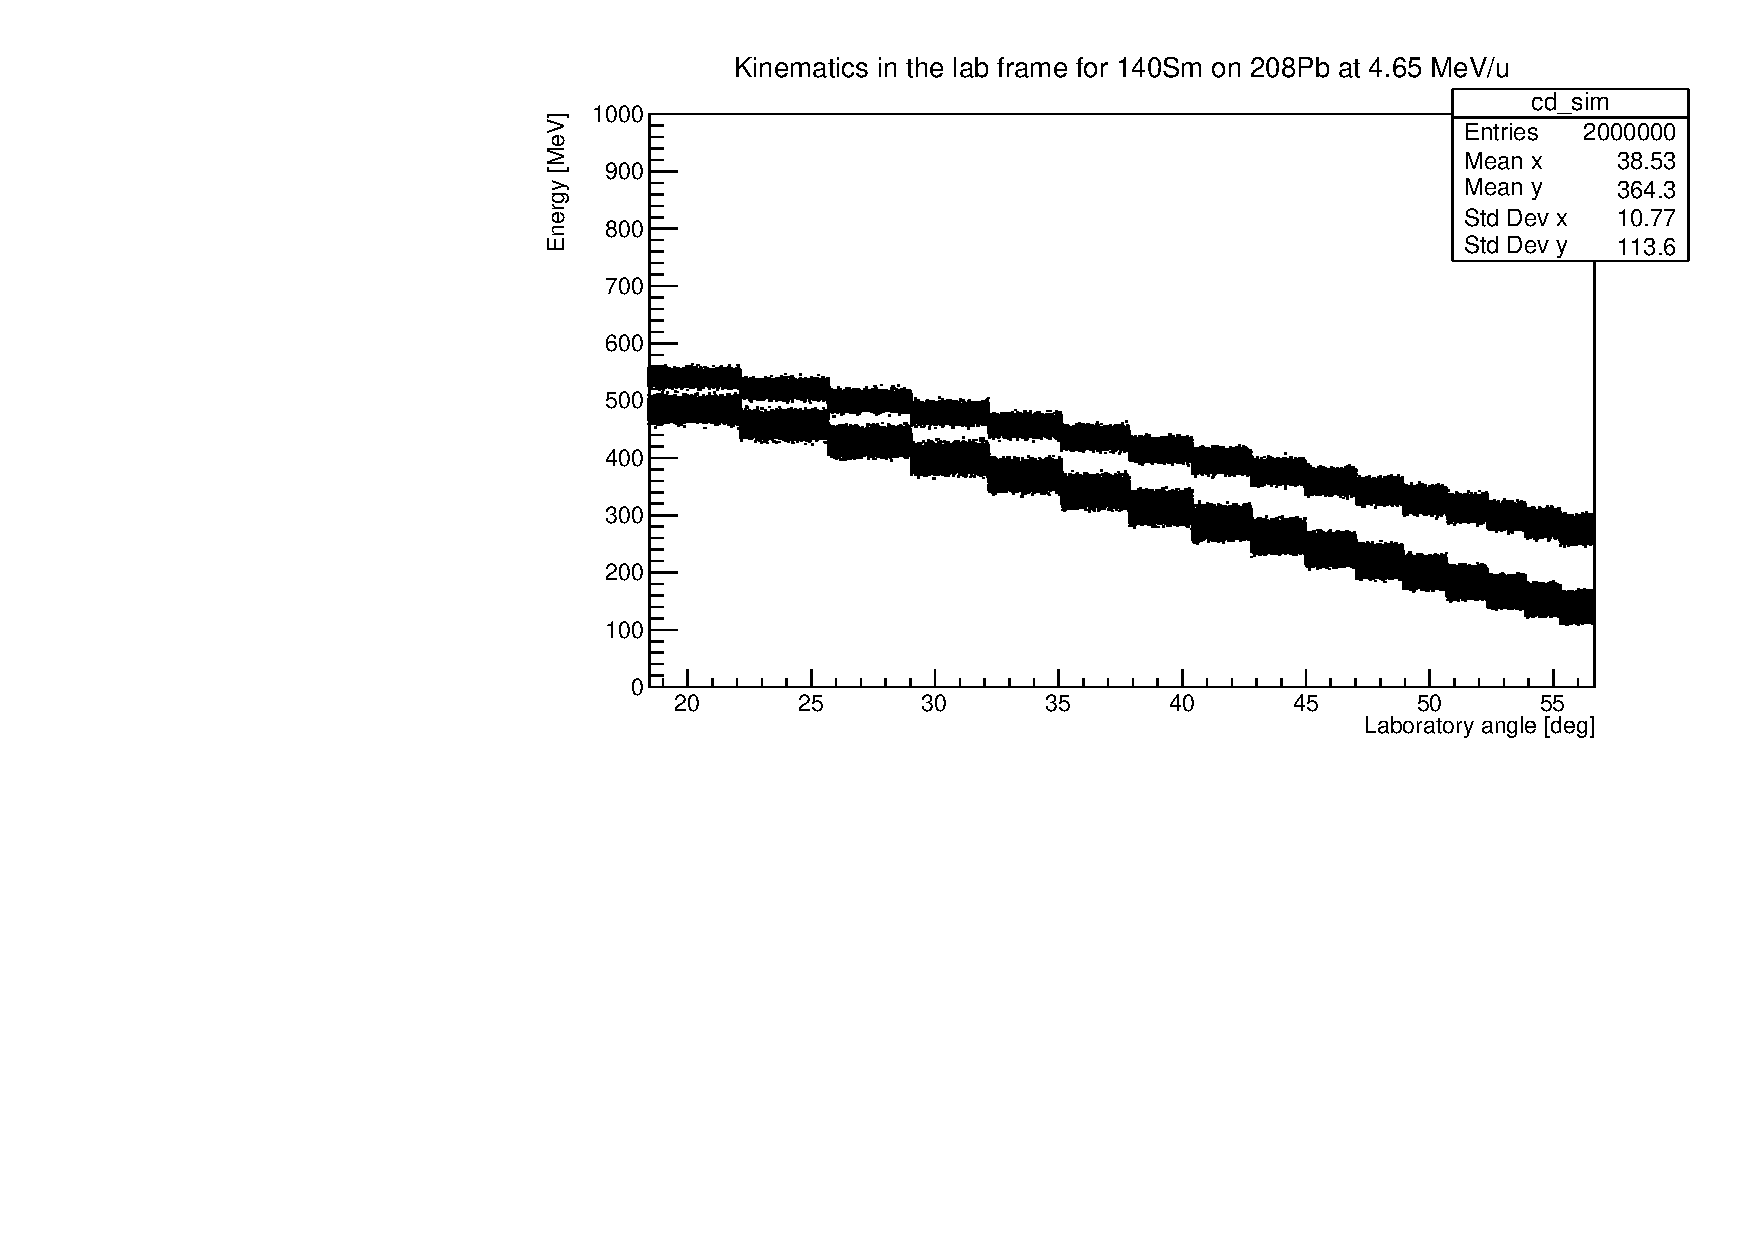
\includegraphics[width=\linewidth]{../Plots/simulation/kin_140Sm_208Pb.pdf}
\end{figure}

\textcolor{Magenta}{Tilbakemelding: \newline 
explain figure: Sm/Pb inner ring, Sm/Pb outer ring \newline
simulation does not consider cross sections: in simulation all angles are equally probable. The corresponding figure from your data looks therefore quite different.
}


\textbf{--- \textcolor{red}{Mail from Liam started} ---} \newline
"the source has a thickness of 1.23 mm, which needs to be factored in so that the CD to target distance is the CD to source distance PLUS the source thickness, i.e. 25.78 mm + 1.23 mm =  27.01 mm. 
This is very close to the 26.98 mm you got from us in August. 
\textcolor{red}{I think that the source data was reanalysed since the original blog entry, giving the 0.03 mm difference!}" \newline
\textbf{--- \textcolor{red}{Mail from Liam ended} ---} \newline


Terminal: Simulation: 140Sm on 208Pb:
\begin{lstlisting}[language=sh]
$ cd GitHub/Miniball/kinsim
$ root
root [0] .L kinsim3.cc+
root [1] kinsim3(62, 82, 140, 208, 1.4, 4.65, 0.02, 1.0, 0.6, 26.98, false, 1e6, "../SRIM")
\end{lstlisting}


kinsim3 function:
\begin{lstlisting}[language=c++]
void kinsim3( int Zb, int Zt, double Ab, double At, double thick /* mg/cm^2 */, double Eb /* MeV/u */,
    double dEb = 0.1 /* MeV/u */, double Ex = 1.0 /* MeV */, double res = 0.6 /* % */,
	double cd_dist = 28.0 /* mm */, bool flat = false /* angular distribution? */,
	long Nevts = 1E6, string srim_dir = "../srim" )
\end{lstlisting}

\bigskip

\textcolor{red}{Say something about SRIM files.}

\bigskip



\section{Calibration}

\textcolor{Magenta}{Tilbakemelding: \newline 
start with explaining the general idea for the calibration: \newline 
determine centroids of peaks in spectra, compare with simulations (kinematics, energy loss) to get linear coefficients (gain + offset). You could show spectra for 2 rings: one where it is ok to get the 2 centroids for Sm and Pb, and one where it is difficult $\rightarrow$ use additional data (Ni?) \newline
Sectors: cover wide angular range $\rightarrow$ no sharp peaks  \newline
Solution: gate on rings to see peaks in sectors and calibrate. \newline
Idea: \newline
1. produce spectra \newline
2. set thresholds: example, explain criteria \newline
3. find calibration coefficients $\rightarrow$ see above \newline
explain strategy, show examples... \newline
4. time calibration 
}


My goal of the calibration was to make a program that could automatically fit the plots i needed, but it became more and more manual labor. 
Because of the shape of the data peaks, it demands very much individual care. 
This I could not do with a automatic program. 
The downfall of the automatic centroid collector came when trying it on the back detectors. 

The total amount particle front detectors to calibrate is 4 quadrants * 16 rings = 64 front detectors 

back detectors: 4 quadrants * 12 strips = 48 back detectors


but to do this, one need all the centroids of the peaks from both sides:

front: 64 detectors * 2 peaks/ring = 128 centroids

back: 48 detectors * 2 peaks/ring * 16 rings =  1536 centroids 

total centroids to collect: 1664 centroids (this I did not want to do manually)

Full calibration with 16 rings and 12 back strips. We had to remove the innermost ring. 



\textcolor{red}{MOVE THE BELOW TO APPENDIX?}

\textcolor{Magenta}{Tilbakemelding: \newline 
up to you. I would do like this: \newline
very technical things about scripts etc. I would move to an appendix. If it helps understanding what you did, I would leave it in the text.
}

For each file converted with MedToRoot, the program makes four files; OffBeam, OnBeam, OnBeamBackground and Scaler. The file we are interested in for analysis is the OnBeam file. 

First all of the interesting files are converted with the M2R.sh script. 
\begin{lstlisting}[language=sh]
$ cd /Users/trondwj/GitHub/MasterThesis/Scripts/sorting 
$ ./M2R.sh Sm
\end{lstlisting}

Then the OnBeam files from M2R.sh is run through using Treebuilder in the AQ4S.sh script. 

\begin{lstlisting}[language=sh]
$ cd /Users/trondwj/GitHub/MasterThesis/Scripts/sorting 
$ ./AQ4S.sh Sm user TB
$ mv Sm_user-TreeBuilder-2019-04-10.root ../../Sorted_data/
\end{lstlisting}


After the sorting, I moved the file to a folder of sorted data, and gave the relative path in the setup\_Sm.txt file in Scripts/plotting/ used as input in the MultiPlot.cpp script. 
Using the MultiPlot.cpp script, the ADC time offsets can be extracted by the following commands
\begin{lstlisting}[language=sh]
$ cd /Users/trondwj/GitHub/MasterThesis/Scripts/plotting
$ root
root [0] .L MultiPlot.cpp++
root [1] check_ADC_time_offsets("setup_Sm.txt")
\end{lstlisting}
or they can be manually reached by
\begin{lstlisting}[language=sh]
$ cd /Users/trondwj/GitHub/MasterThesis/Sorted_data
$ root Sm_user-TreeBuilder-2019-04-10.root
root [1] new TBrowser()
\end{lstlisting}
and in the browser, the histograms named tdiff\_gp\_\textit{i} (where \textit{i} is a number between 0 and 3) will lie under all the folders. The peaks of these plots have the interesting x-value. Zooming into the peaks, it is very clear what value it is. These values are provided in the calibration file under ADC time offsets (ticks). These values can change depending on the amount of data sorted, so it is wise to double check them.

After the peak values have been collected, they should be written into the calibration file
\begin{lstlisting}[language=sh]
# ADC time offsets (ticks)
adc_0.TimeOffset:  0
adc_1.TimeOffset:  -2
adc_2.TimeOffset:  -3
adc_3.TimeOffset:  5
\end{lstlisting}

\begin{figure}[ht]
	\centering
	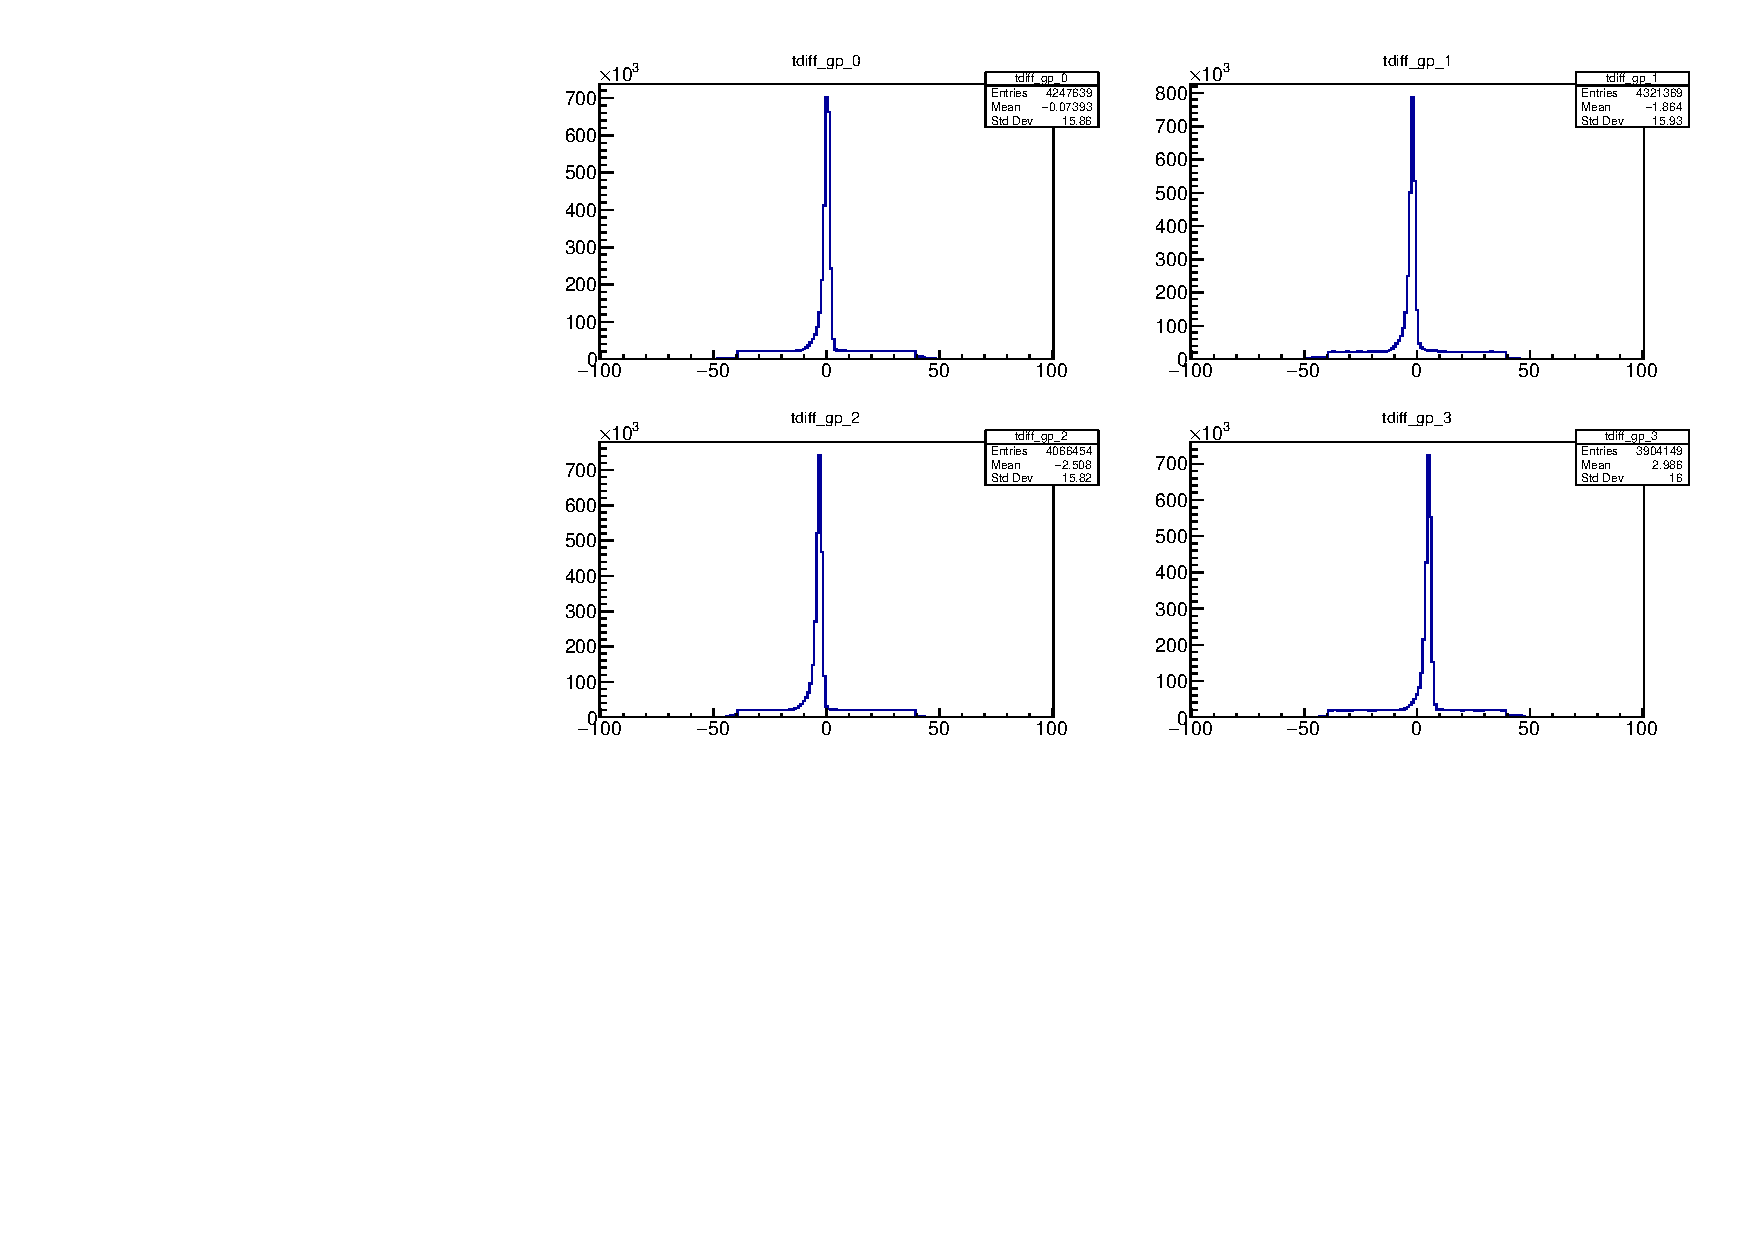
\includegraphics[width=\textwidth]{../Plots/plotting/tdiff_gp_0-3-user.pdf}
	\caption{ADC time offsets.}
	\label{fig:ADC_dt}
\end{figure}

\textcolor{Magenta}{Tilbakemelding: \newline 
one time spectrum per quadrant?
}


\textcolor{red}{HUSK:} Si noe om ADC time offsets + Threshold. Og at man må se på det tidlig, så resortere.


M2R.sh $\rightarrow$ AQ4S.sh$\rightarrow$ check time offset $\rightarrow$ threshold $\rightarrow$ AQ4\_fit() $\rightarrow$ particle-calibration.py $\rightarrow$  ADC\_generator.py $\rightarrow$ copy the calibration from the terminal and paste into calibration file 

\textcolor{Magenta}{Tilbakemelding: \newline 
need to explain the time spectra: start - stop \newline
purpose: align time spectra so that you can set a prompt time gate. \newline
$\rightarrow$ correlate $\gamma$-rays with particles.
}


Simulation fit $\rightarrow$ AQ4\_fit() $\rightarrow$ particle-calibration.py $\rightarrow$  ADC\_generator.py $\rightarrow$ copy the calibration from the terminal and paste into calibration file 

Visualize plots using ROOT and the scripts. 



Skriv om scriptene som er lagd, og at det var litt vanskelig å automatisere kalibreringen. Hvis det skulle vært gjort måtte vi funnet en funksjon med "negatively skewed distribution" or "negative skewness" (right modal), en "left skewed function" (most data is more than the mean). 


I log-skala ser dette mer Gaussisk ut, men det er ikke det i non-log skala. 


Back detector calibration: There are just too much individual differences to calibrate the back detectors with a simple script given a range for all 12 back strips. I found out this way to late. There isn't any range to rule them all, at least since the fitting function can behave very strange given a too small or too big range.



\textbf{--- \textcolor{red}{Mail from Liam begins} ---}

"You might have to investigate the threshold a little bit. The continuum of events at low energy comes from charge sharing between the strips. For these very heavy ions, the total amount of charge deposited gets split between neighbouring strips of the CD. The code does performs some tricks to try and recover the correct energy and position, but that depends on counting the number of strips that fire. Therefore, if the threshold is too low you will include "pedestal" events and it will get things wrong. If the threshold is too high, you will miss some events that have charge sharing and get the wrong energy for your particle. 

The key spectra to look at are "part" and "cd\_debug". The latter counts how many particles have X strips fired on the front side and Y strips fired on the back side.

If you have too many cd\_debug events = 3, then your thresholds are too low. If you have a large continuum/background in the "part" spectrum, your thresholds are too high. Best thing to do is play about with different values.

Bin 20 is when no particle can be found, because there is no energy registered in either the front or the back strips. This can only happen when the front energy is below the software threshold that you set and the back energy is either in a broken strip or is also below the software threshold. Likely it is some noise events or charge sharing that comes below the threshold.

\textcolor{red}{The major problem with the online calibration is that a number of the back strips have the wrong gains}, but it otherwise looks quite good. Have you identified which strips these are, by comparing the gains between the 'online' and 'user' calibrations? You could maybe correct those strips as an intermediate step and see how things look.

the source has a thickness of 1.23 mm, which needs to be factored in so that the CD to target \textcolor{red}{distance is the CD} to source distance PLUS the source thickness, i.e. 25.78 mm + 1.23 mm =  27.01 mm. This is very close to the 26.98 mm you got from us in August. I think that the source data was reanalyzed since the original blog entry, giving the 0.03 mm difference!"

For the centroids, it is very hard to tell in log scale how precise you are with the automatic fitting. I zoomed in on one example (attached) and you can see that the black lines do not really represent the centroid in this instance (black lines too low in energy). Because of the complex peak shapes, it is very hard to do this with automatic fitting it seems. 

It honestly might be better to simply hover your mouse over the correct "feature" of the peak, be it the centroid or the maximum, and compare that. The fitting just doesn't seem reliable.

If you do not have the cdpad option selected, then there will be no particle events, because they come in the CD. The -s flag is for adding particles which come without a gamma-ray and the add back flag is for adding Compton scattered events together in the Miniball clusters. 

What you observe around channel number 20 in the ADC events is the so-called pedestal. There is a single common gate for the each ADC (containing channels from one CD quadrant). Therefore, when there is an event in one strip of the CD all channels are readout,  but the channels without a real event read a "zero" energy. These are the events in the pedestal. You should define your threshold for each ADC channel to be above this peak. You are simply zoomed in to the wrong range. Maybe try with log scale on the y-axis and you will see that there should be a cut off at low-energy. After a correct calibration is applied (as you can see for adc\_1\_19 in your example), this pedestal will be calibrated out of the physical energy range.

The nominal calibration will be quite good for most detectors in a certain energy range, because it is designed to be that way. The gains of each DGF are matched during the setup of the experiment so that the online analysis is more straightforward. However, there are some non-linearities and drifting offsets and gains over time that have to be corrected for with a proper calibration using the 133Ba/152Eu source data. 

\textbf{--- \textcolor{red}{Mail from Liam ended} ---}

\textcolor{Magenta}{Tilbakemelding: \newline 
I presume that charge sharing is only considered if 2 firing strips are neighbors?
}

\textbf{Pedestal}

The pedestal is like a massive statue in front of the interesting data. 


We use a threshold to cut away the pedestal.

\begin{figure}[ht]
	\centering
	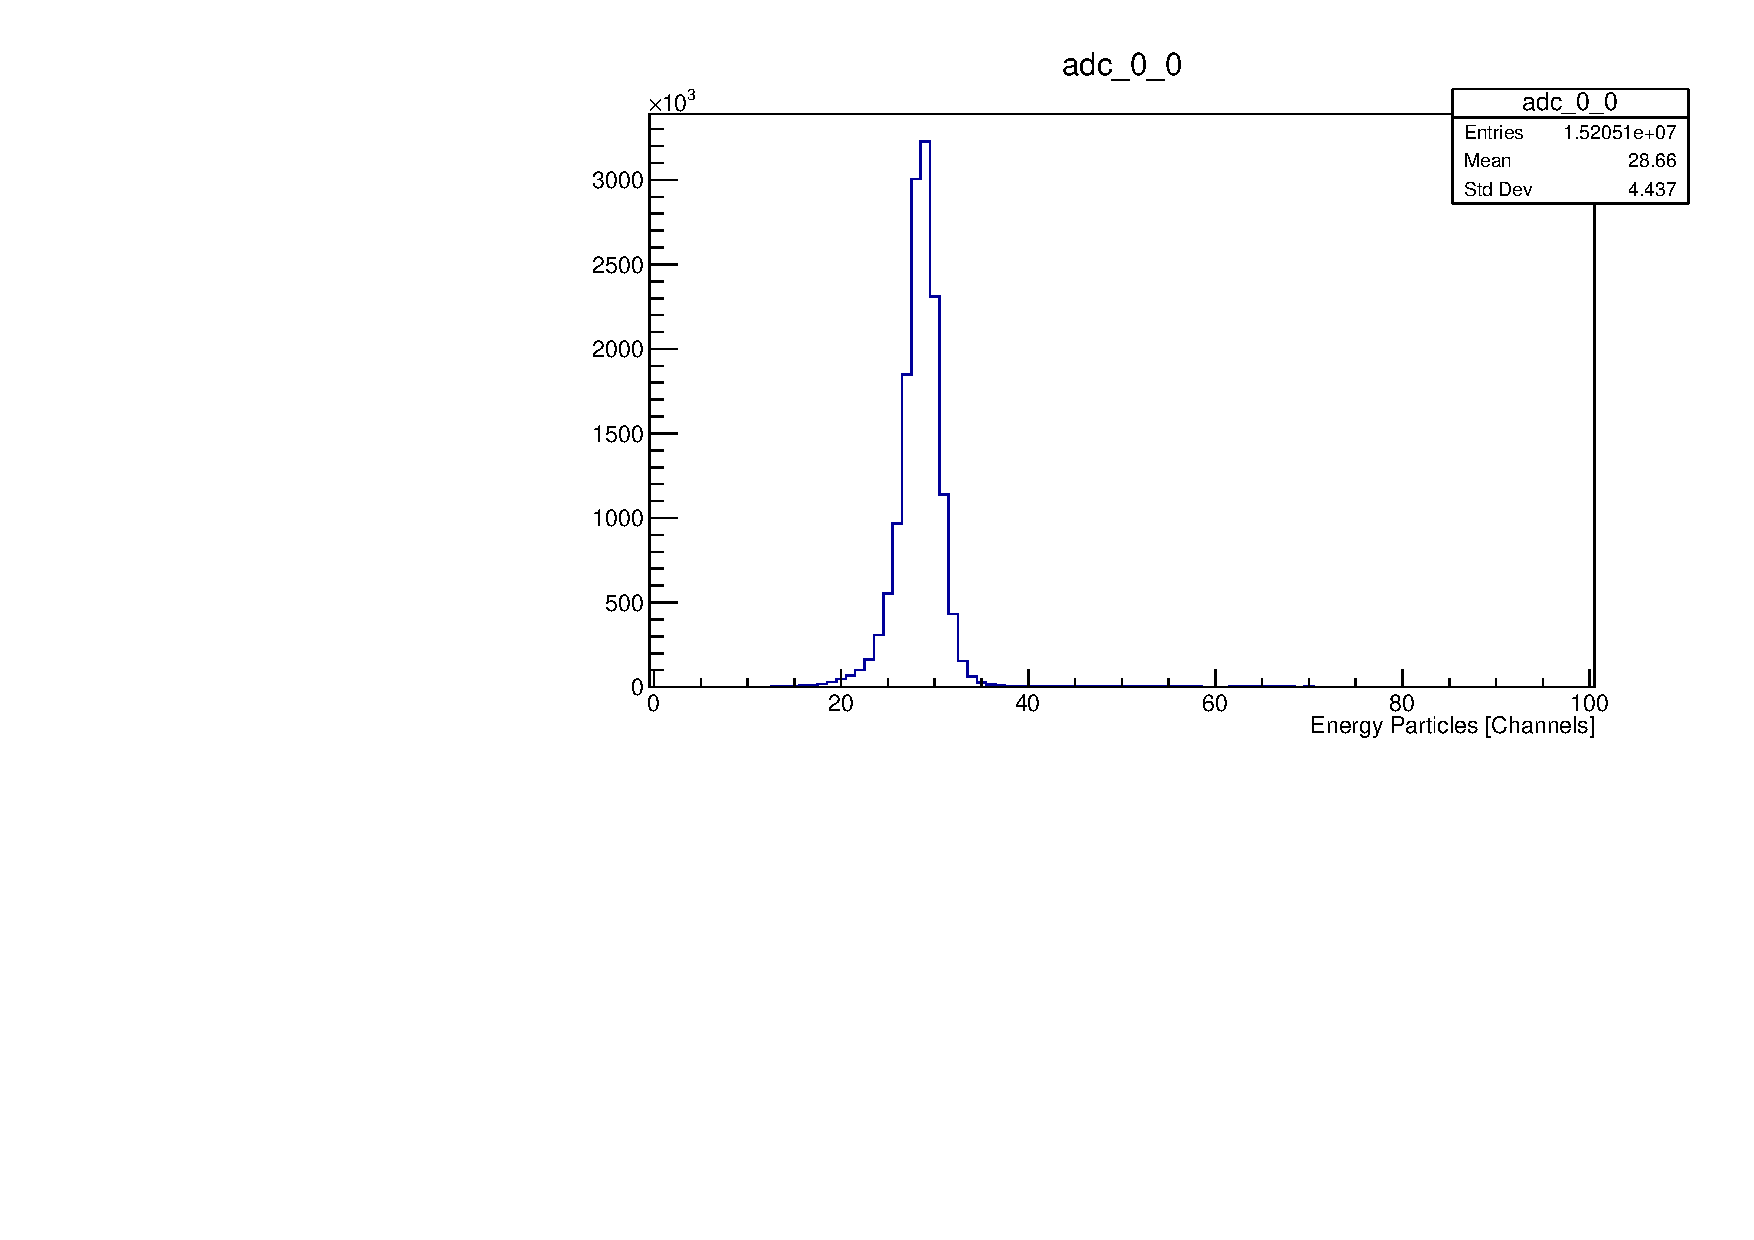
\includegraphics[width=\textwidth]{../Plots/plotting/Pedestal_Q1_f1.pdf}
	\caption{Pedestal Q1, f1.}
	\label{fig:Pedestal_f}
\end{figure}

\begin{figure}[ht]
	\centering
	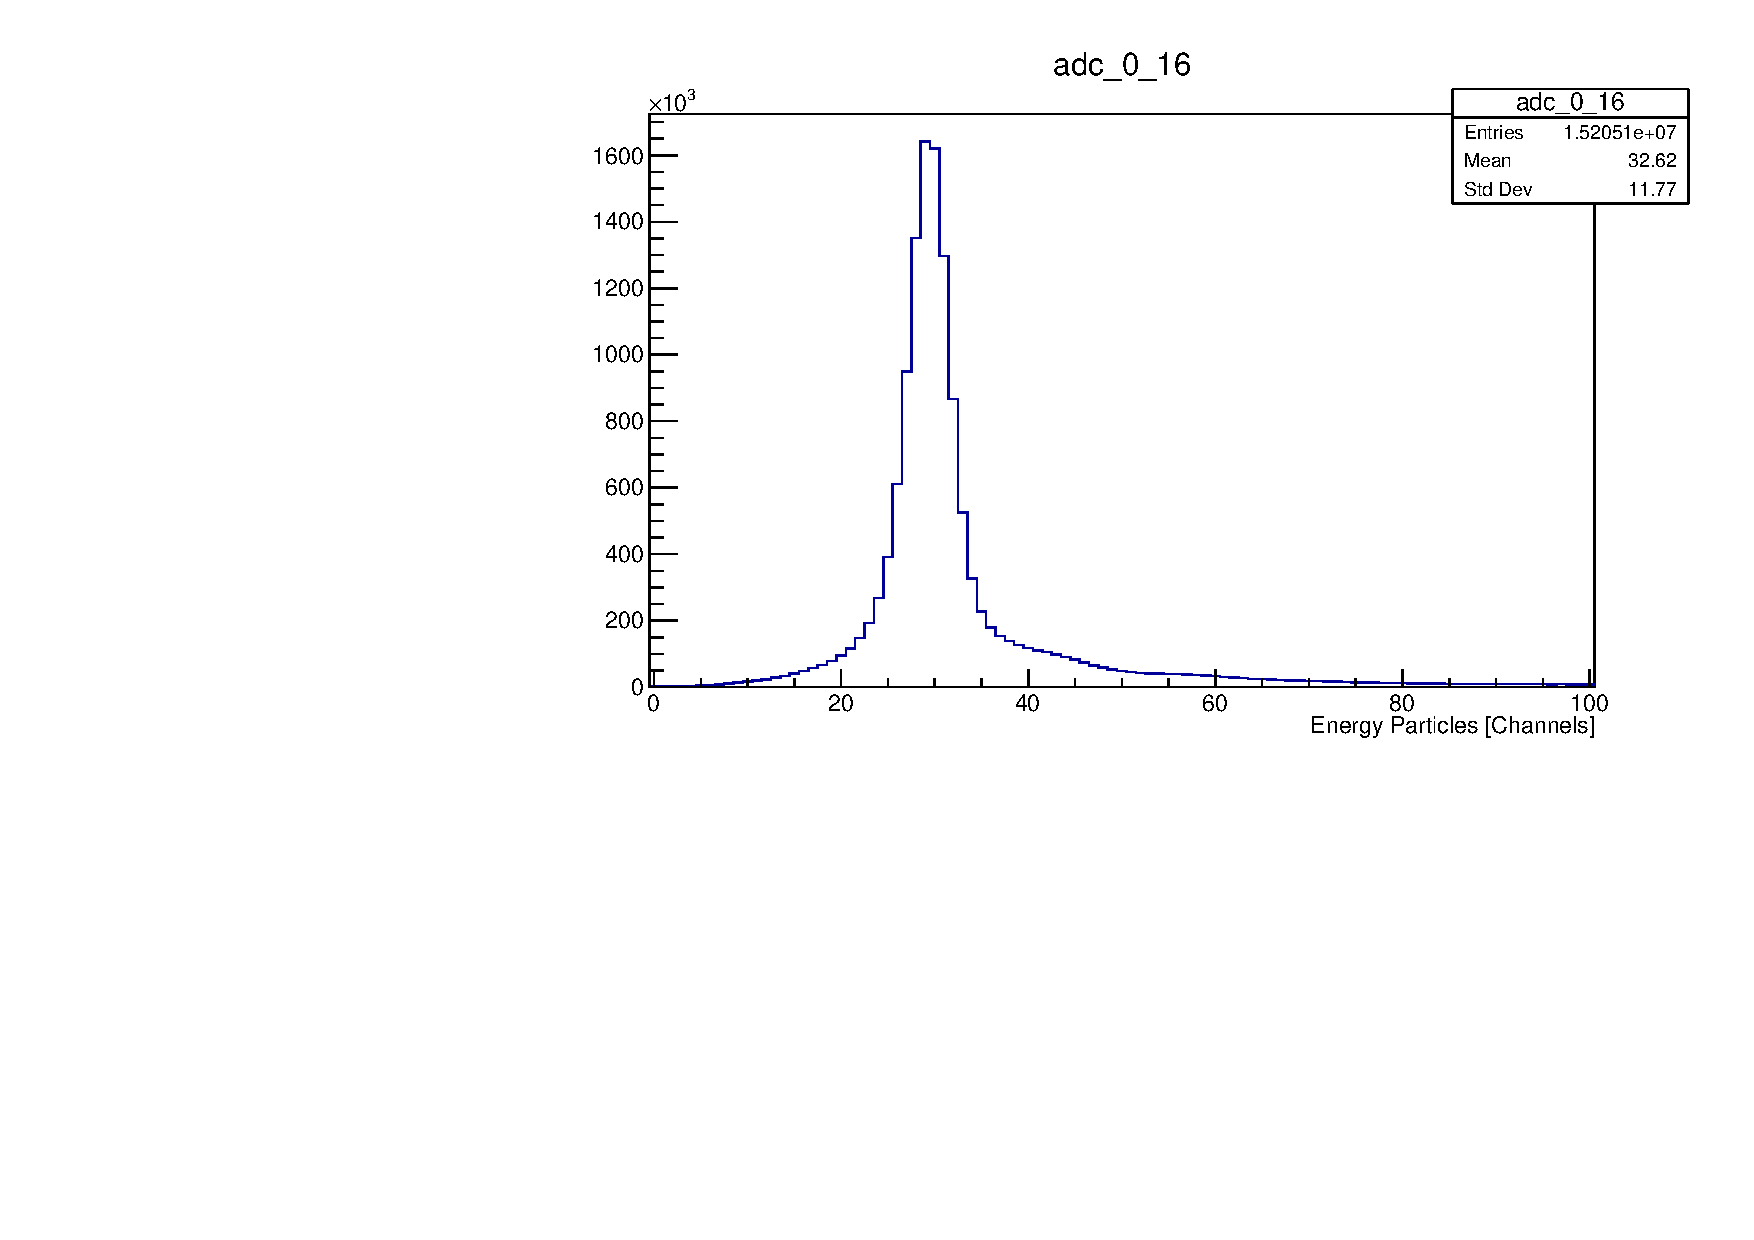
\includegraphics[width=\textwidth]{../Plots/plotting/Pedestal_Q1_b1.pdf}
	\caption{Pedestal Q1, b1.}
	\label{fig:Pedestal_b}
\end{figure}



\textbf{Threshold}

* Threshold (forskjellig i log/ikke-log skala)

Using a logarithmic y-axis, the threshold value will decrease very much. So don't use that. 

\textcolor{Magenta}{Tilbakemelding: \newline 
easier to set thresholds on lin. scale.
}

Threshold: The code has a default threshold of 100, but in some cases this is too much and some cases this is not enough. So for each adc channel, the threshold can be set. We don't want to include the "pedestal". Charge sharing.
Won't cut too much or too little..

\begin{figure}[ht]
	\centering
	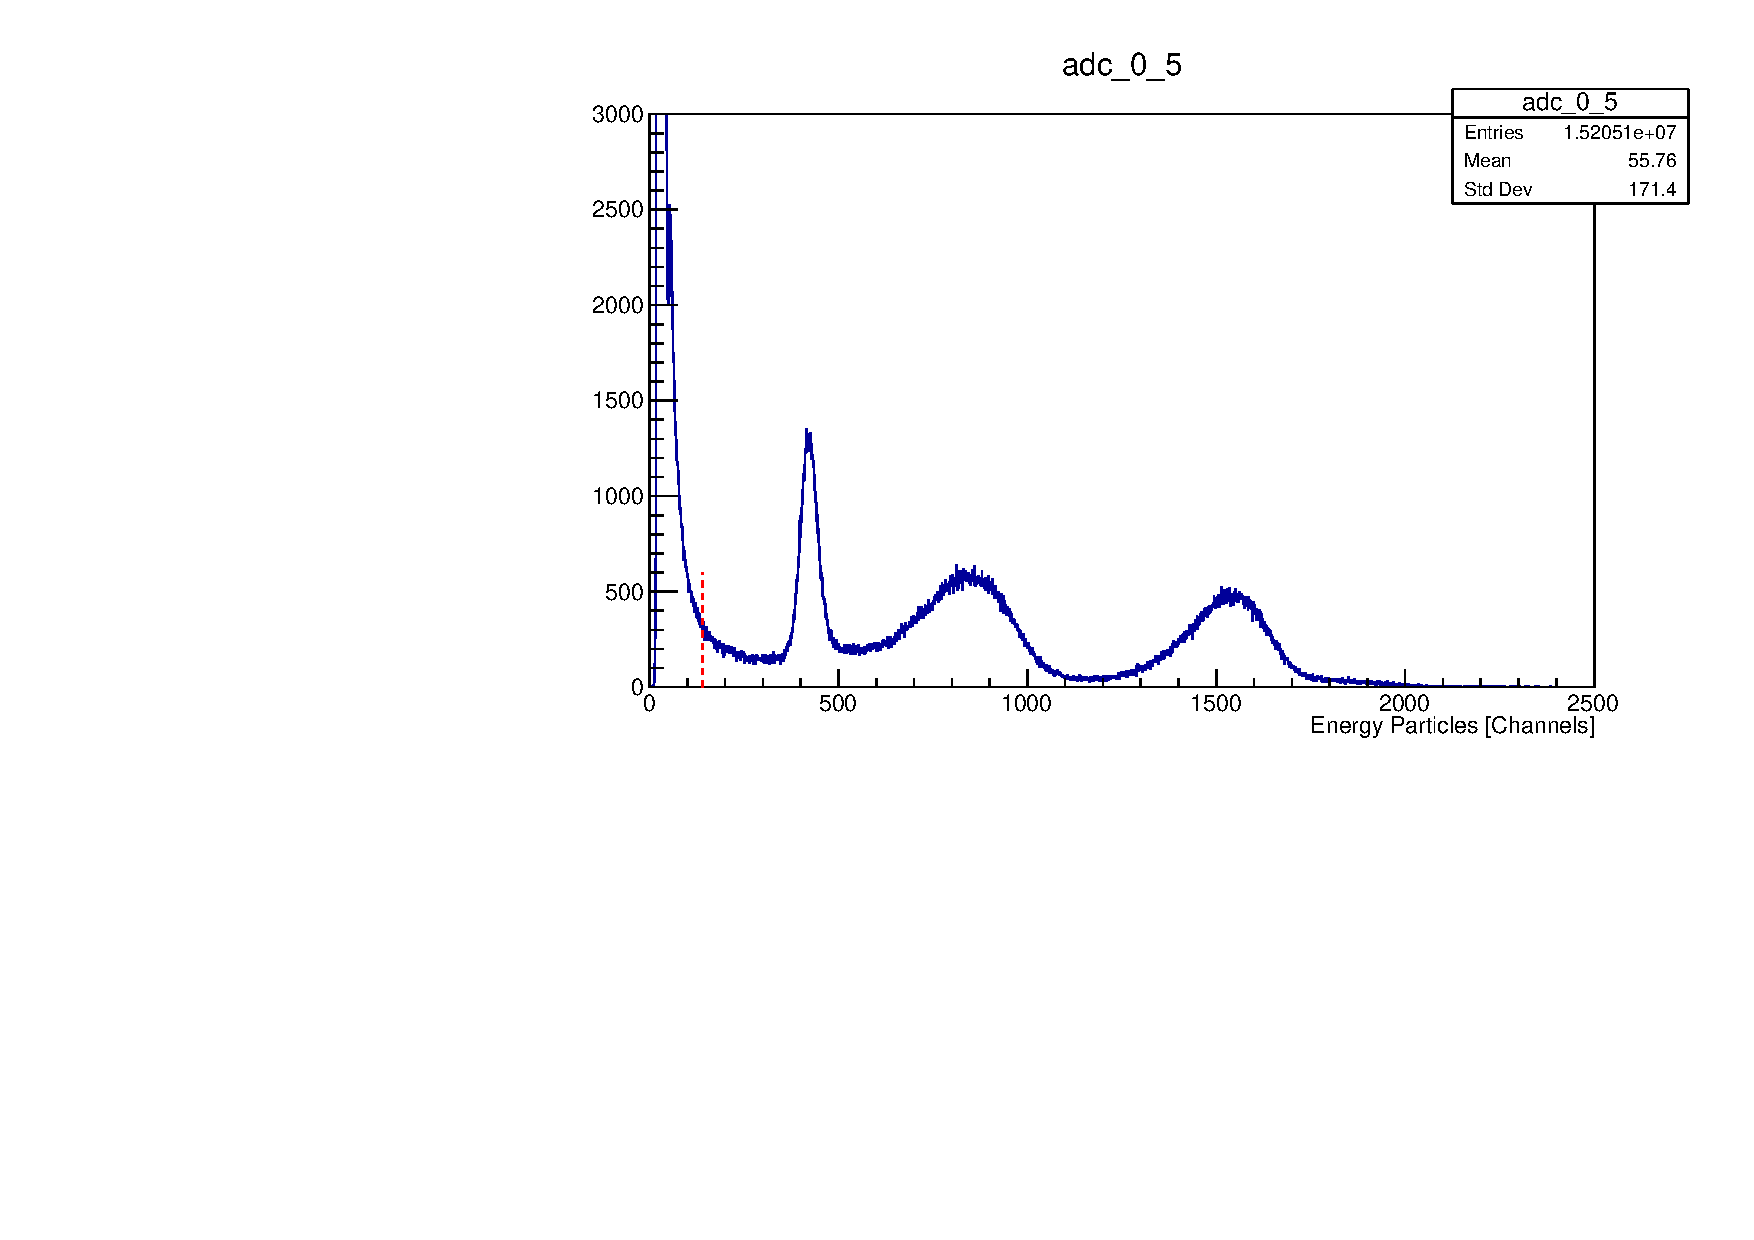
\includegraphics[width=\textwidth]{../Plots/plotting/Threshold_Q1_f6.pdf}
	\caption{Threshold Q1, f6.}
	\label{fig:Threshold_f}
\end{figure}


\begin{figure}[ht]
	\centering
	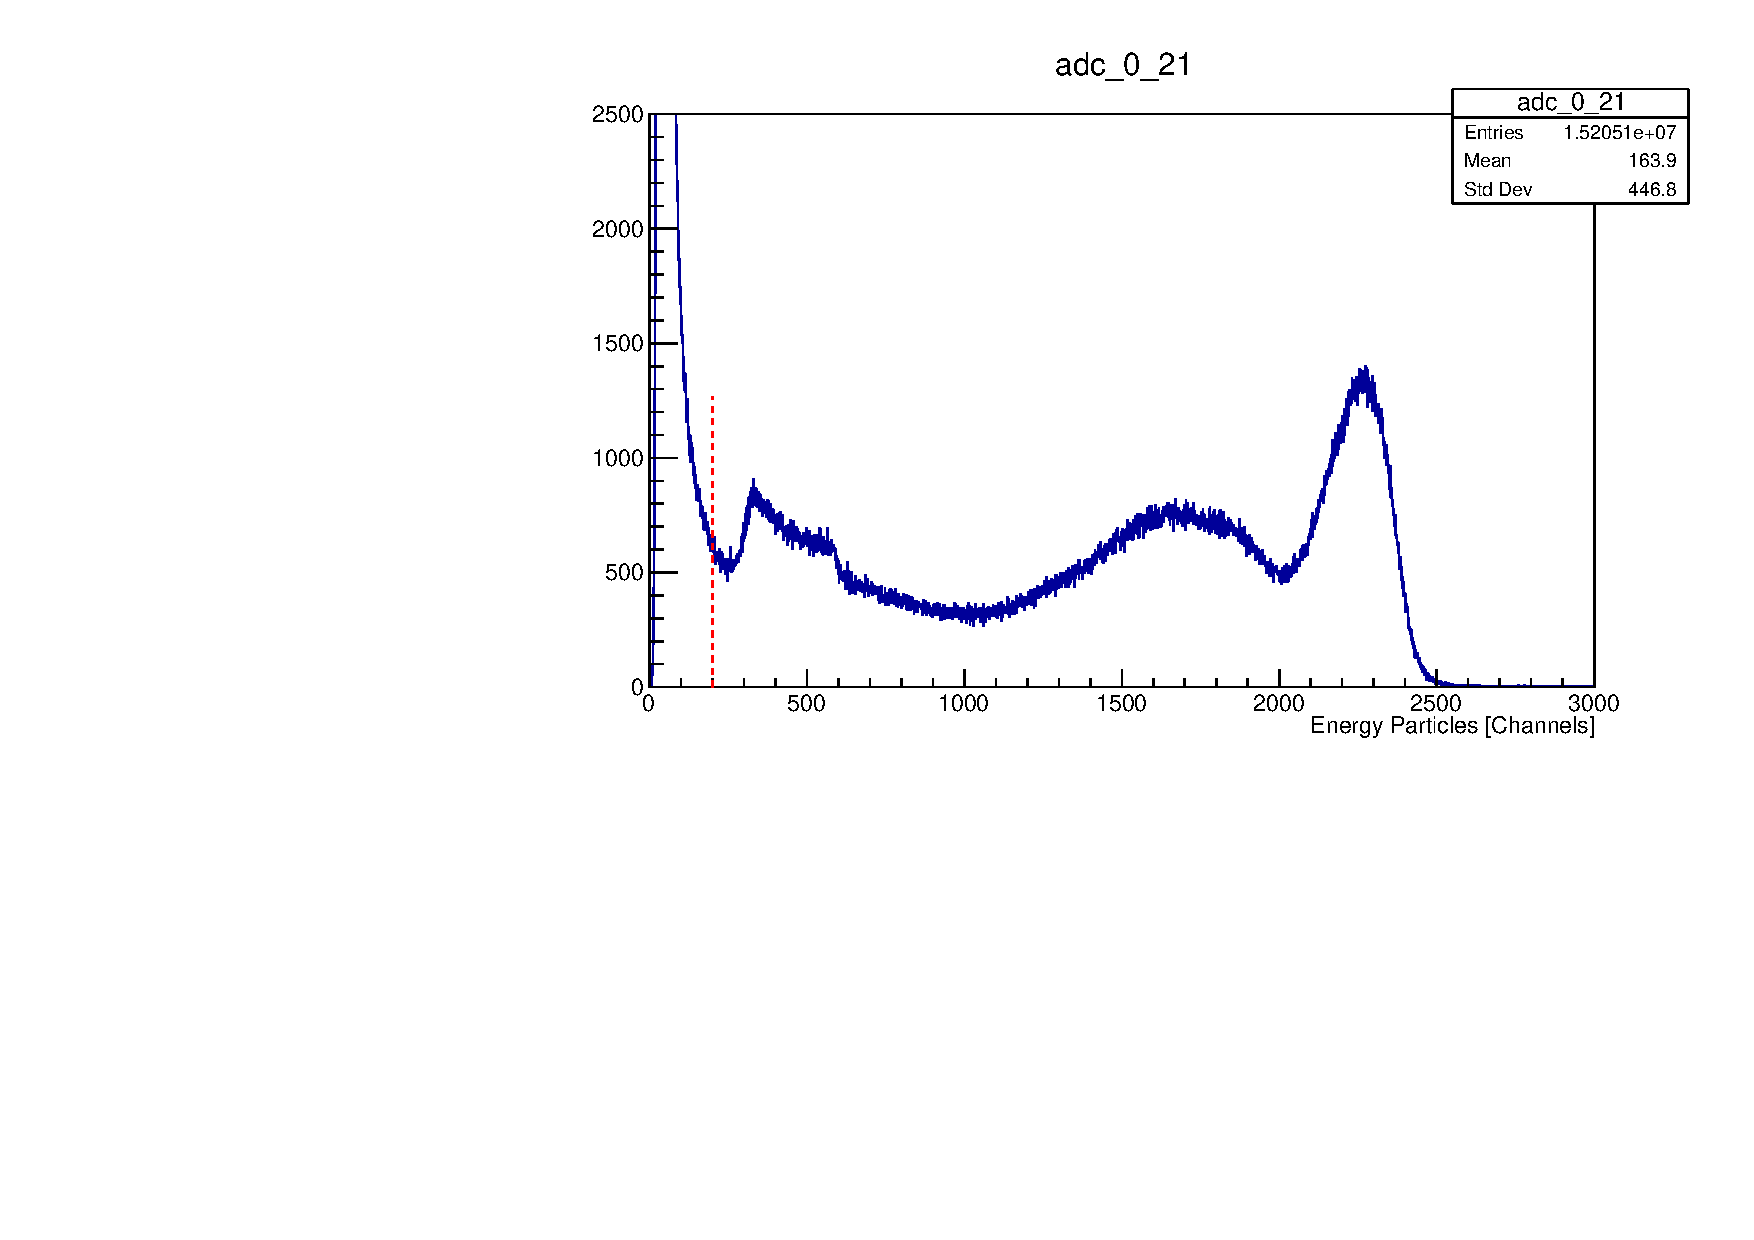
\includegraphics[width=\textwidth]{../Plots/plotting/Threshold_Q1_b6.pdf}
	\caption{Threshold Q1, b6.}
	\label{fig:Threshold_b}
\end{figure}


\textbf{CD debug:}

\begin{lstlisting}[language=sh]
$ cd /Users/trondwj/GitHub/MasterThesis/Scripts/plotting 
$ root
root [0] .L MultiPlot.cpp++
root [1] check_cd_debug("setup_Sm.txt")
\end{lstlisting}


\begin{figure}[ht]
	\centering
	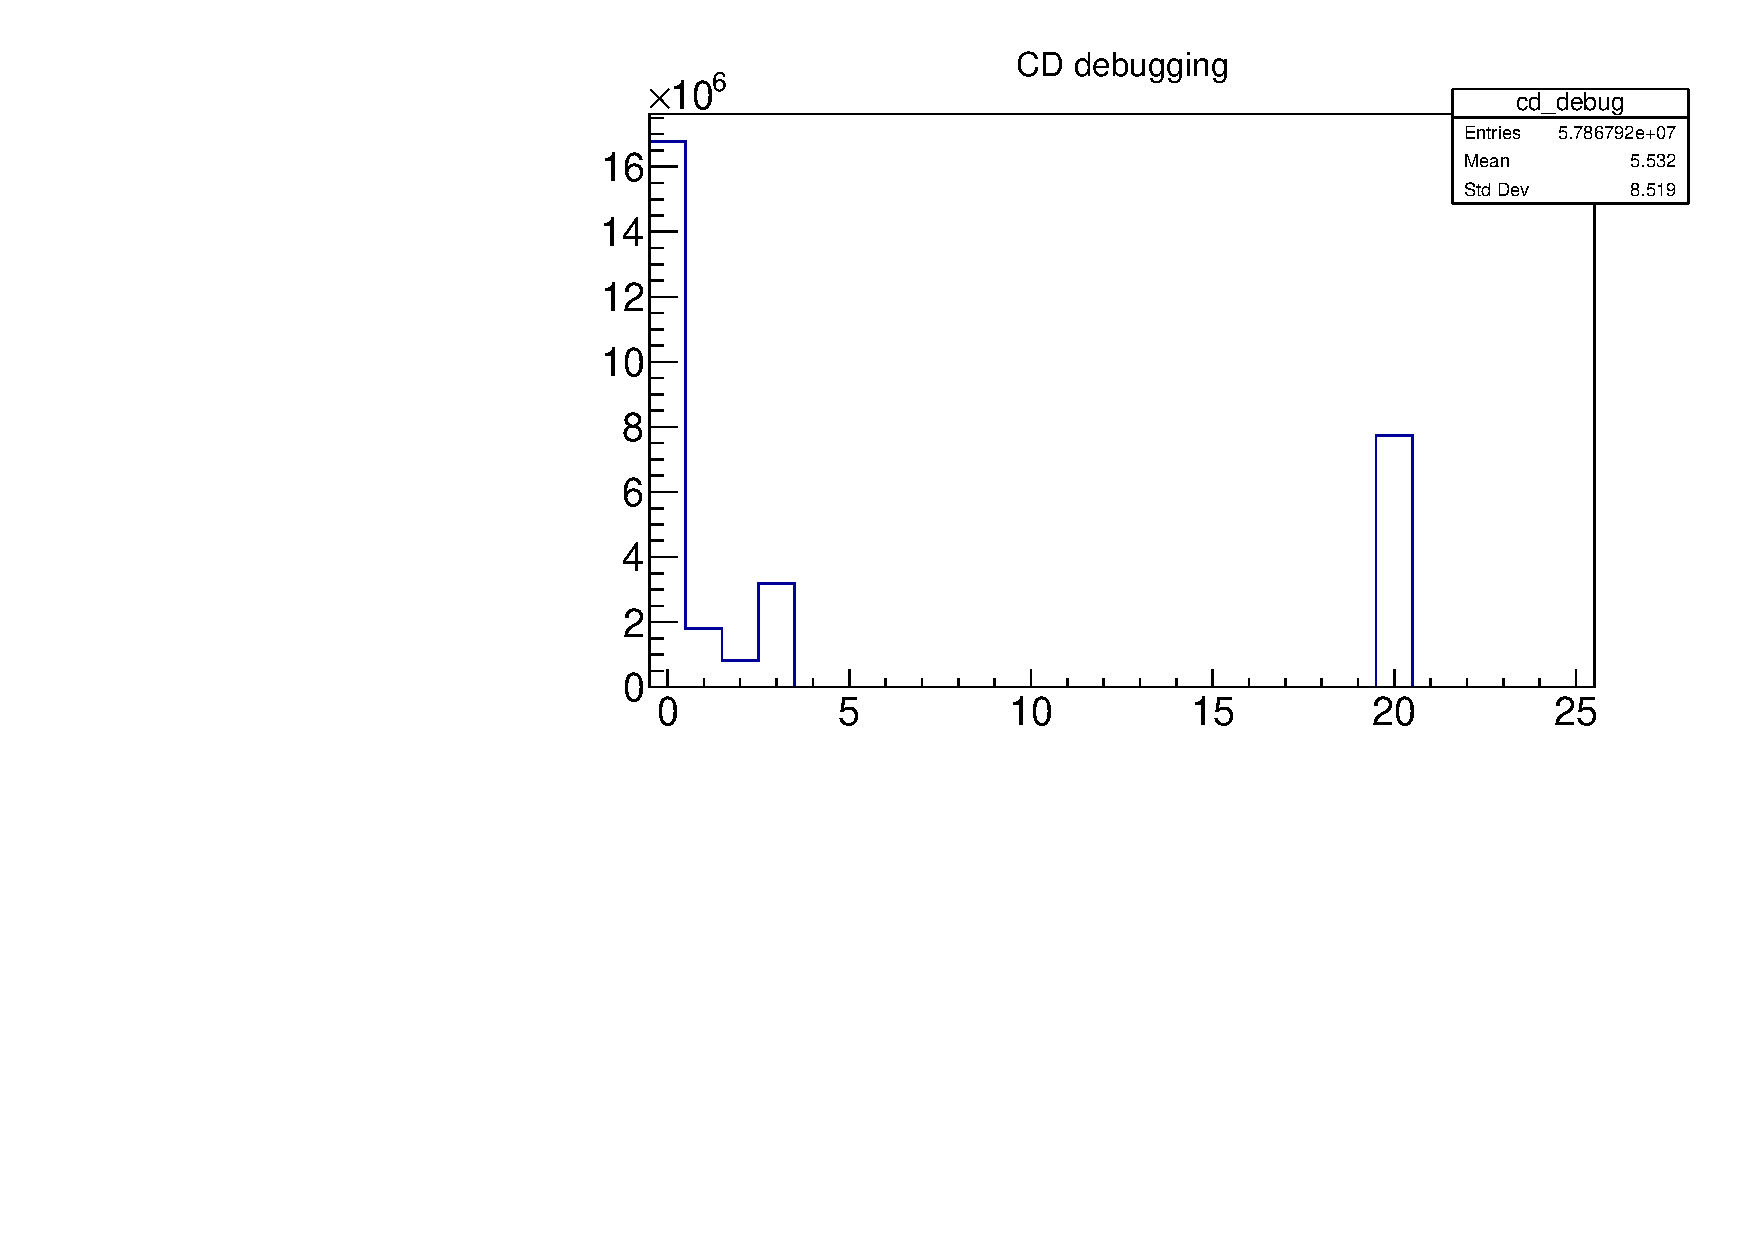
\includegraphics[width=\textwidth]{../Plots/plotting/cd_debug-user.pdf}
	\caption{CD debugging.}
	\label{fig:CD_debug}
\end{figure}


\subsection{Particle detector}


\subsubsection{User calibration}
ADC: Analog to digital converter (Mesytec)

TDC: Time to digital converter

DSSSD: Double-Sided Silicon Strip Detector $\implies$ CD

must remove the inner ring from data analysis because of damage

\begin{align*}
	\text{gain} = \frac{E_{\text{Sm}} - E_{\text{Pb}}}{Ch_{\text{Sm}} - Ch_{\text{Pb}}}
\end{align*}

\begin{align*}
	\text{offset} = E_{\text{Sm}} - \text{gain} \cdot Ch_{\text{Sm}}
\end{align*}
in keV.

\textcolor{red}{Hvis man har flere sentroider bruker man bare lineær regresjon. Gjelder spesielt for baksiden!}

\begin{figure}[ht]
	\centering
	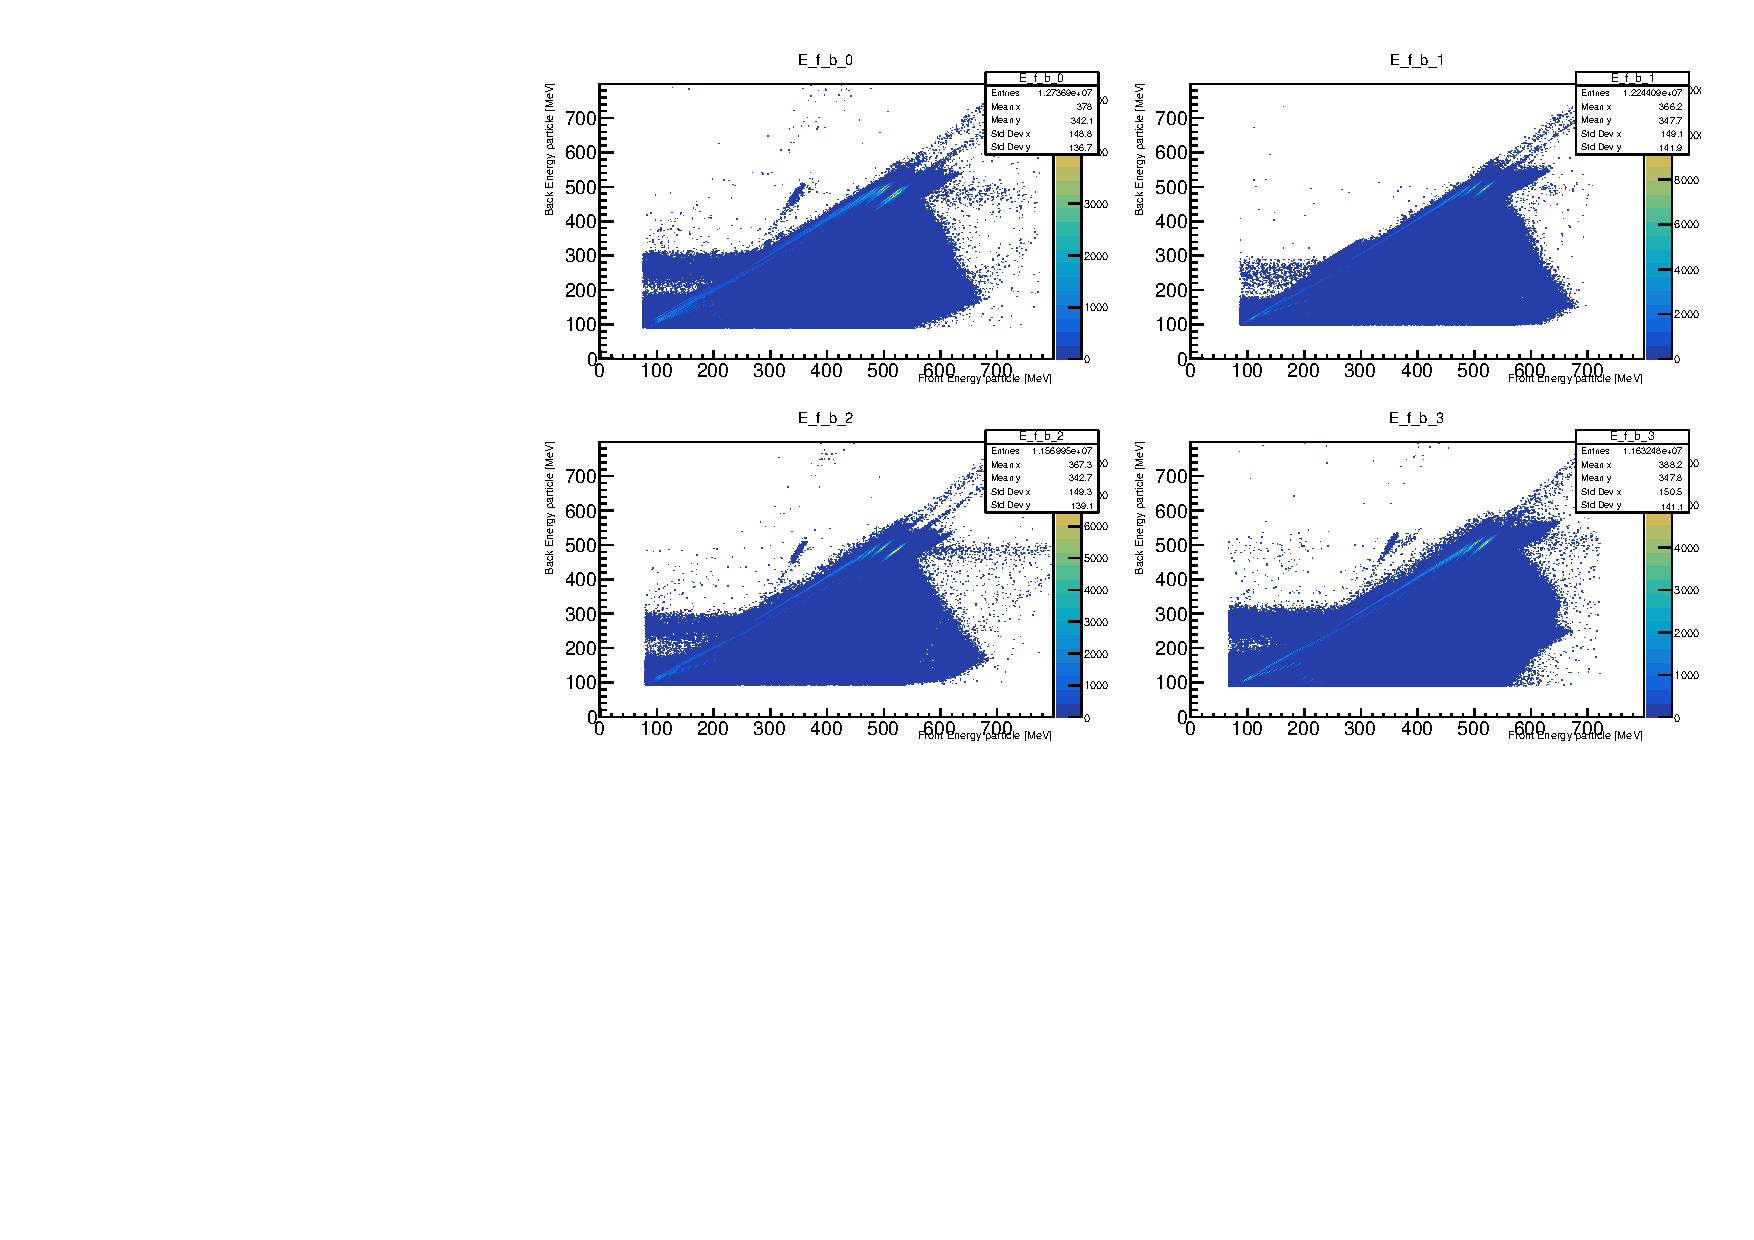
\includegraphics[width=\textwidth]{../Plots/plotting/E_f_b_Q1-4-user-new-cal.pdf}
	\caption{User calibration.}
	\label{fig:cal_user}
\end{figure}



\subsubsection{Online calibration}


\begin{figure}[ht]
	\centering
	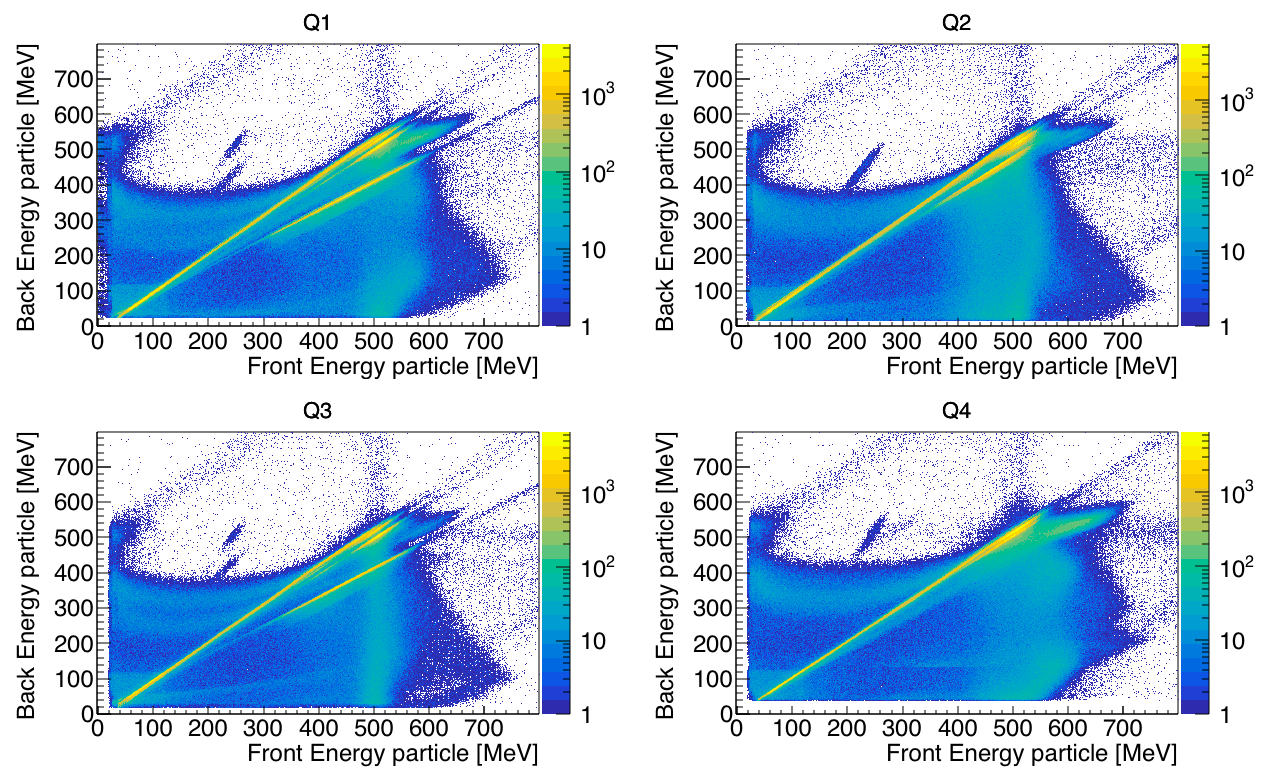
\includegraphics[width=\textwidth]{../Plots/plotting/E_f_b_Q1-4-online.pdf}
	\caption{Online calibration.}
	\label{fig:cal_online}
\end{figure}



\subsection{Gamma detectors}

DGF: Digital \ga~ finder

addback, singles, ...



\section{Doppler correction}





% ----------------------------------------------------------------------------------------------------------------------% ----------------------------------------------------------------------------------------------------------------------


\chapter{Experimental results}


% ----------------------------------------------------------------------------------------------------------------------% ----------------------------------------------------------------------------------------------------------------------


\chapter{Discussion}

Level scheme (from Klintefjord?)\newline

\textcolor{Magenta}{Tilbakemelding: \newline
at some point you should show the level scheme. \newline
$\bullet$ motivation: to explain what is known, and which transition probabilities you want to measure.  \newline
Perhaps also to explain what theory predicts. \newline
$\bullet$ discussion: if you get \ga-spectrum for \Sm ~$\rightarrow$ to explain what you see.}


\begin{figure}
	\centering
	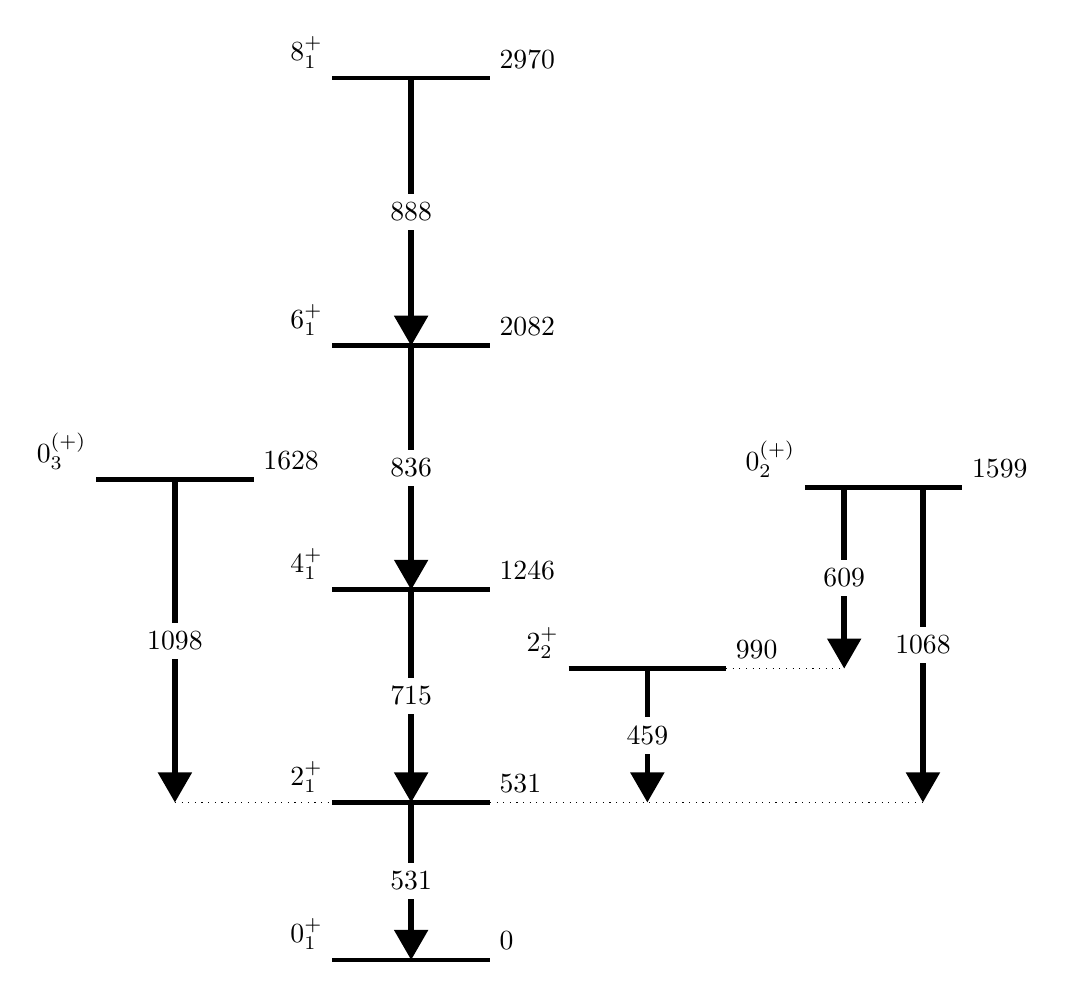
\begin{tikzpicture}[
    level/.style = { ultra thick, black },
    connect/.style = { dotted, black },
    notice/.style = { draw, rectangle callout, callout relative pointer={#1} },
    label/.style = { text width=2cm }
    ]
    %%% Picture made by normalizing energy to the 2+ state (531) and choosing it to be 
    %%% 2 units of y in height.

    %%%
    %%% Ground state band
    %%%
    % Levels, states, energy
    \foreach \level / \state / \energy in {0/0_1^+/0, 2/2_1^+/531, 4.7/4_1^+/1246, 7.8/6_1^+/2082, 11.2/8_1^+/2970}
      { 
        \draw[level] (0,\level) -- (2,\level);
        \node at (0,\level) [anchor=south east] {$\state$};
        \node at (2,\level) [anchor=south west] {$\energy$};
      }
    % Gamma transitions
    \foreach \endlevel / \startlevel / \gamma in {0/2/531, 2/4.7/715, 4.7/7.8/836, 7.8/11.2/888}
      { 
        \draw[line width=2pt, ->, >=triangle 60] (1,\startlevel) -- node[fill=white] {\gamma} (1,\endlevel);
      }
    % Dotted lines
    \draw[connect] (-2,2) -- (0,2) (2,2) -- (7.5,2);
    %\draw[connect] (-2,11.2) -- (0,11.2) (2,11.2) -- (4,11.2);
    
    %%%
    %%% Left band
    %%%
    % Lower left band
    \coordinate (levelleft)  at (-3,6.1);
    \coordinate (levelright) at (-1,6.1);
    \draw[level] (levelleft) -- (levelright);
    \node at (levelleft)  [anchor=south east] {$0_3^{(+)}$};
    \node at (levelright) [anchor=south west] {1628};
    \draw[line width=2pt, ->, >=triangle 60] (-2,6.1) -- node[fill=white] {1098} (-2,2);
    %% Higher left band
    %\foreach \level / \state / \energy in {12.1/10^+/3211, 13.8/12^+/3653, 16.6/14^+/4404, 20.3/16^+/5398}
    %  { 
    %    \draw[level] (-3,\level) -- (-1,\level);
    %    \node at (-3,\level) [anchor=south east] {$\state$};
    %    \node at (-1,\level) [anchor=south west] {$\energy$};
    %  }
    %% Gamma transitions
    %\foreach \endlevel / \startlevel / \gamma in {12.1/13.8/442, 13.8/16.6/751, 16.6/20.3/994}
    %  { 
    %    \draw[line width=2pt, ->, >=triangle 60] (-2,\startlevel) -- node[fill=white] {\gamma} (-2,\endlevel);
    %  }
    %% First gamma transition
    %\draw[line width=2pt, ->, >=triangle 60] (-2,12.1) -- node[left=3pt] {241} (-2,11.2);

    %%%
    %%% 1st right band
    %%%
    % Lower 1st right band
    \coordinate (levelleft)  at (3,3.7);
    \coordinate (levelright) at (5,3.7);
    \draw[level] (levelleft) -- (levelright);
    \node at (levelleft)  [anchor=south east] {$2_2^+$};
    \node at (levelright) [anchor=south west] {990};
    \draw[line width=2pt, ->, >=triangle 60] (4,3.7) -- node[fill=white] {459} (4,2);
    % Dotted lines
    \draw[connect] (levelright) -- (6.5,3.7);
    %% Higher 1st right band; levels, states, energy
    %\foreach \level / \state / \energy in {11.9/10^+/3172, 14.3/12^+/3791, 18.5/14^+/4914}
    %  { 
    %    \draw[level] (3,\level) -- (5,\level);
    %    \node at (3,\level) [anchor=south east] {$\state$};
    %    \node at (5,\level) [anchor=south west] {$\energy$};
    %  }
    %% Gamma transitions
    %\foreach \endlevel / \startlevel / \gamma in {11.9/14.3/619, 14.3/18.5/1123}
    %  { 
    %    \draw[line width=2pt, ->, >=triangle 60] (4,\startlevel) -- node[fill=white] {\gamma} (4,\endlevel);
    %  }
    %% First gamma transition
    %\draw[line width=2pt, ->, >=triangle 60] (4,11.9) -- node[right=4pt] {202} (4,11.2);

    %%%
    %%% 2nd right band
    %%%
    \coordinate (levelleft)  at (6,6);
    \coordinate (levelright) at (8,6);
    \draw[level] (levelleft) -- (levelright);
    \node at (levelleft)  [anchor=south east] {$0_2^{(+)}$};
    \node at (levelright) [anchor=south west] {1599};
    \draw[line width=2pt, ->, >=triangle 60] (7.5,6) -- node[fill=white] {1068} (7.5,2);
    \draw[line width=2pt, ->, >=triangle 60] (6.5,6) -- node[fill=white] {609} (6.5,3.7);    
\end{tikzpicture}
	\caption{Level scheme for \Sm. Adapted from Klintefjord.}
	\label{fig:levels}
\end{figure}




% ----------------------------------------------------------------------------------------------------------------------% ----------------------------------------------------------------------------------------------------------------------

\chapter{Summary and outlook}

Future work: Better calibration of particle detectors (online not perfect). Take into account the shape of the peaks $\implies$ calibrate the particle detectors manually.. Takes a lot of time! But maybe less than trying to fit all in a script? Had I just known...


\textcolor{red}{Fra oppgaveteksten:} \newline
determine Coulomb excitation yields. These yields will then, in a second step, be compared to theoretical calculations and transition probabilities and quadrupole moments will be extracted using chi-square minimization procedures.


GOSIA and GOSIA2 analysis?

\url{https://www.pas.rochester.edu/~cline/Gosia/Gosia_Manual_20110609.pdf}

% ----------------------------------------------------------------------------------------------------------------------% ----------------------------------------------------------------------------------------------------------------------




% ----------------------------------------------------------------------------------------------------------------------% ----------------------------------------------------------------------------------------------------------------------

\begin{appendices}

\chapter{Symbol list}

\begin{table}[h]
  \centering
  \caption{Table of symbols with explanations.}
    \begin{tabular}{ll}
        \hline
        T$_{1/2}$ & Half-life \\
        \hline
    \end{tabular}
    \label{tab:symbols}
\end{table}


\chapter{Acronyms and abbreviations}

\begin{table}[ht] 
	\centering 
	% Data for the Acronyms and abbreviations table
\begin{tabular}{ll}
    \hline
    ADC         &  Analog to Digital Converter                                \\
    bash        &  Bourne-Again SHell                                         \\
    CERN        &  European Council for Nuclear Research                      \\ 
                &  (in French: Conseil Européen pour la Recherche Nucléaire)  \\
    CD          &  Compact Disc                                               \\
    COULEX      &  COULomb EXcitation                                         \\
    DAQ         &  Data AcQuisition                                           \\
    DGF         &  Digital Gamma Finder                                       \\
    DSSSD       &  Double Sided Silicon Strip Detector (also known as CD)     \\
    GPS         &  General Purpose Separator                                  \\
    HRS         &  High Resolution Separator                                  \\
    HIE-ISOLDE  &  High Intensity and Energy upgrade at ISOLDE                \\
    HPGe        &  High Purity Germanium                                      \\
    ISOL        &  Isotope Separator On Line                                  \\
    ISOLDE      &  ISOL DEvice                                                \\
    LINAC       &  LINear ACcelerator                                         \\
    MBS         &  Multi Branch System                                        \\
    MED         &  MBS Event Data (also known as Miniball Event Data)         \\
    MAR\belowbaseline[-2pt]{a}B\stackinset{l}{3pt}{b}{-3pt}{O}{O}\,U     
                &  MBS And ROOT Based Online/Offline Utility                  \\
    PSB         &  Proton Synchrotron Booster                                 \\
    REX         &  Radioactive beam EXperiment                                \\
    EBIS        &  Electron Beam Ion Source                                   \\
    REXEBIS     &  Radioactive beam EXperiment Electron Beam Ion Source       \\
    REXTRAP     &  Radioactive beam EXperiment TRAP                           \\
    REX-ISOLDE  &  Radioactive beam EXperiment at ISOLDE                      \\
    RIB         &  Radioactive Ion Beam                                       \\
    RILIS       &  Resonance Ionization Laser Ion Source                      \\
    SRIM        &  Stopping and Range of Ions in Matter                       \\
    TDC         &  Time to Digital Converter                                  \\
    \hline
\end{tabular}
\label{tab:acro}

\end{table}


\chapter{Source code}
The sorting and analysis code used in this thesis has been developed at CERN-ISOLDE and can be found at \url{https://github.com/Miniball/MiniballCoulexSort}

The code for theoretical predictions of energy used in the calibration was developed by Liam Gaffney who is working at ISOLDE and has to do with analysis of data from Miniball and ISS. kinsim can be found here \url{https://github.com/lpgaff/kinsim}

Some calibration code is based on the codes of Ville Virtanen and Liam Gaffney. 

Other code/scripts have been written by the author. C++ / Python.

\begin{table}[h]
  \centering
  \caption{Table of source code.}
    \begin{tabular}{ll}
        \hline
        Name/Link & Description \\
        \hline
         \href{https://github.com/Miniball/MiniballCoulexSort}{MiniballCoulexSort} & Sorting and analysis code \\
         \href{https://github.com/lpgaff/kinsim} & Kinematic simulation \\
        \hline
    \end{tabular}
    \label{tab:code}
\end{table}


\chapter{Connecting MiniballCoulexSort with ROOT}
To connect MiniballCoulexSort with ROOT you need them to share their libraries with each other. This is done with a dynamic loader. You can find out more here: \url{https://root.cern.ch/root/htmldoc/guides/users-guide/ROOTUsersGuide.html#file-system.rootrc}. 

You have to make a \textbf{.rootrc} file in your home folder on your computer. In the \textbf{.rootrc} file you want to write something like this 
\begin{lstlisting}[language=sh]
Unix.*.Root.DynamicPath:    .:</Users/trondwj/GitHub/ROOT-framework/build/lib>:/Users/trondwj/GitHub/Miniball/MiniballCoulexSort/lib:
\end{lstlisting}
This should all be in one line. The first part is to tell the system to use the dynamic loader of ROOT to connect the given paths that follow. In my case the lib folder of the ROOT install was at 
\begin{lstlisting}[language=sh]
/Users/trondwj/GitHub/ROOT-framework/build/lib
\end{lstlisting}
and the lib folder of the MiniballCoulexSort was at
\begin{lstlisting}[language=sh]
/Users/trondwj/GitHub/Miniball/MiniballCoulexSort/lib
\end{lstlisting}
These paths is totally individual, and you will probably not have it in the same place. Therefore these paths must be changed to fit your system. 

After making the file you either have restart the terminal or you can source the file by writing this in the terminal
\begin{lstlisting}[language=sh]
$ source ~/.rootrc
\end{lstlisting}


\chapter{Running ROOT and MiniballCoulexSort from anywhere in the terminal}
To run ROOT or the different scripts of MiniballCoulexSort anywhere in the terminal, you have to edit your \textbf{.bash\_profile} file [.bash\_profile on MacOS, .bashrc on Linux]. In my \textbf{.bash\_profile} I used this 
\begin{lstlisting}[language=sh]
# Run ROOT from anywhere
export ROOTSYS=$HOME/GitHub/ROOT-framework/build
export PATH=$ROOTSYS/lib:$PATH
export PATH=$ROOTSYS/bin:$PATH
export DYLD_LIBRARY_PATH=$ROOTSYS/lib:$DYLD_LIBRARY_PATH

# Run MiniballCoulexSort from anywhere
export DYLD_LIBRARY_PATH=$HOME/GitHub/Miniball/MiniballCoulexSort/lib:$DYLD_LIBRARY_PATH
export PATH=$HOME/GitHub/Miniball/MiniballCoulexSort/lib:$PATH
export PATH=$HOME/GitHub/Miniball/MiniballCoulexSort/bin:$PATH
\end{lstlisting}
The DYLD\_LIBRARY\_PATH is used on Mac only. On other systems, use \newline LD\_LIBRARY\_PATH. You need to locate the lib and bin folders for both ROOT and MiniballCoulexSort and change them to fit your system, and in addition you need the build folder of your ROOT install.


\chapter{Other appendicies}
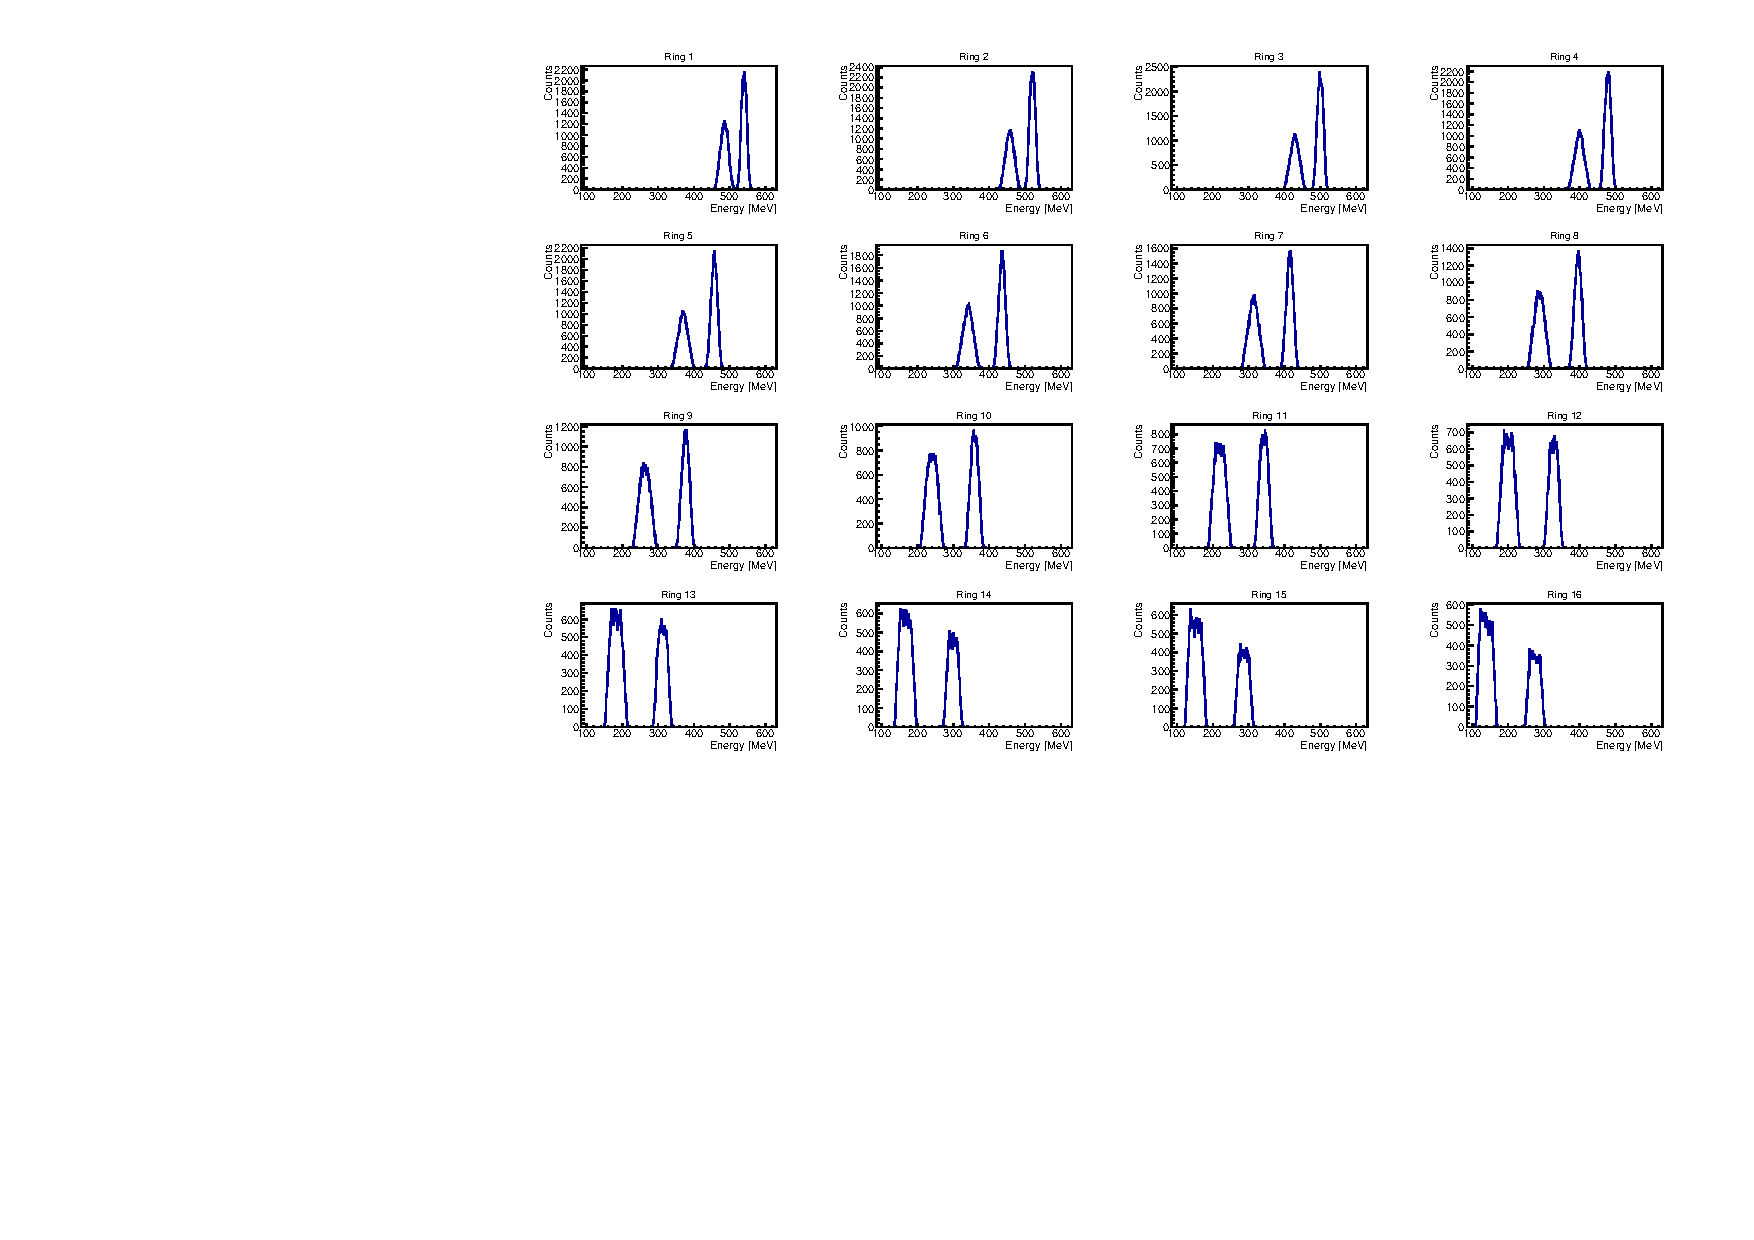
\includepdf[pages={-}, angle=270]{../Plots/simulation/cd_sim_all.pdf}


\end{appendices}



%\bibliographystyle{unsrtnat}
\bibliographystyle{mybibstyle} %my own bibstyle to set first names to one letter + unsrtnat

\bibliography{/Users/trondwj/GitHub/MasterThesis/Thesis/Mendeley/ISOLDE.bib,/Users/trondwj/GitHub/MasterThesis/Thesis/References/web_references.bib}


\end{document}